%\documentclass[a4paper,superscriptaddress,11pt]{quantumarticle}
\documentclass[aps,twocolumn,longbibliography,english,superscriptaddress]{revtex4-1}
%\documentclass[a4paper,superscriptaddress,11pt]{article}
\pdfoutput=1
\usepackage[colorlinks=true,urlcolor=blue,citecolor=blue,linkcolor=blue]{hyperref}
\usepackage[english]{babel}
\usepackage[utf8]{inputenc}
\usepackage[T1]{fontenc}
\usepackage{amssymb}
\usepackage{tabularx}
\usepackage{upquote}
\usepackage{subcaption}
%\usepackage{multicol}
%\usepackage{caption}
%\usepackage[plain]{algorithm}
\usepackage[ruled, vlined]{algorithm2e}
\usepackage{algpseudocode}
\usepackage{rotating}
%\usepackage{cite}
\usepackage{booktabs}
%\usepackage{unicode-math}
%\usepackage{algorithm}% http://ctan.org/pkg/algorithm
%\usepackage{algpseudocode}% http://ctan.org/pkg/algpseudocode
\usepackage{xcolor}% http://ctan.org/pkg/xcolor
\makeatletter
\newsavebox{\@brx}
\newcommand{\llangle}[1][]{\savebox{\@brx}{\(\m@th{#1\langle}\)}%
  \mathopen{\copy\@brx\kern-0.5\wd\@brx\usebox{\@brx}}}
\newcommand{\rrangle}[1][]{\savebox{\@brx}{\(\m@th{#1\rangle}\)}%
  \mathclose{\copy\@brx\kern-0.5\wd\@brx\usebox{\@brx}}}
\makeatother
\usepackage{bbm}
\usepackage{jlcode}
\usepackage{graphicx}
\usepackage{amsmath,color,amsthm}
\usepackage{mathrsfs}
\usepackage{float}
\usepackage[normalem]{ulem}
\usepackage{indentfirst}
\usepackage{txfonts}
\usepackage[epsilon, tsrm, altpo]{backnaur}

\usepackage{listings}
\lstset{
    language=Julia,
    basicstyle=\ttfamily\footnotesize,
    numberstyle=\scriptsize,
    % numbers=left,
    backgroundcolor=\color{gray!10},
    frame=single,
    tabsize=2,
    rulecolor=\color{black!30},
    title=\lstname,
    %escapeinside={\%(*}{*)},
    breaklines=true,
    breakatwhitespace=true,
    framextopmargin=2pt,
    framexbottommargin=2pt,
    extendedchars=true,
    inputencoding=utf8,
    columns=fullflexible,
}

\tolerance=1
\emergencystretch=\maxdimen
\hyphenpenalty=1000
\hbadness=1000

\makeatletter

%%%%%%%%%%%%%%%%%%%%%%%%%%%%%% User specified LaTeX commands.

%Journal reference.  Comma sets off: name, vol, page, year
\def\journal #1, #2, #3, 1#4#5#6{{\sl #1~}{\bf #2}, #3 (1#4#5#6) }
\def\pr{\journal Phys. Rev., }
\def\prb{\journal Phys. Rev. B, }
\def\prl{\journal Phys. Rev. Lett., }
\def\pl{\journal Phys. Lett., }
%\def\np{\journal Nucl. Phys., }


%%%%%%%%%%%%%%%%%%%%%%%%%%%%%%%%%%%%%%%%%%%%%%%%%%%%%%%%%%%%%%%%%%%%%%%%%%%%%%%%%%%%%%%%%%%%%%%%%%%%%%%%%%%%%%%%%%%%%%%%%%%%%%%%%%%%%%%%%%%%%%%%%%%%%%%%%%%%%%%%%%%%%%%%%%%%%%%%%%%%%%%%%%%%%%%%%%%%%%%%%%%%%%%%%%%%%%%%%%%%%%%%%%%%%%%%%%%%%%%%%%%%%%%%%%%%


%\usepackage{CJK}
%\usepackage[colorlinks, citecolor=blue]{hyperref}
\DeclareMathOperator*{\argmax}{arg\,max}

%%%%%% Shortcut related
\newcommand{\<}{\langle}
\renewcommand{\>}{\rangle}
\newcommand{\out}{{\vx^L}}
\newcommand{\inp}{{\vx^0}}
\newcommand{\cquad}{{{ }_{\quad}}}
\newcommand{\pluseq}{\mathrel{+}=}
\newcommand{\minuseq}{\mathrel{-}=}
\newcommand{\vx}{{\mathbf{x}}}
\newcommand{\vg}{{\mathbf{g}}}
\newcommand{\vp}{{\mathbf{p}}}
\newcommand{\vy}{{\mathbf{y}}}
\newcommand{\Var}{{\mathrm{Var}}}
\newcommand{\Mean}{{\mathrm{E}}}
\newcommand{\vvalue}{{\texttt{value}}}
\newcommand{\grad}{{\texttt{grad}}}
\newcommand{\parameter}{{\texttt{parameter}}}
%%%%%% Convention related
\newcommand{\SWAP}{{\rm SWAP}}
\newcommand{\CNOT}{{\rm CNOT}}
\newcommand{\X}{{\rm X}}
\renewcommand{\H}{{\rm H}}
\newcommand{\Rx}{{\rm Rx}}
\renewcommand{\v}[1]{{\bf #1}}
\newcommand{\dataset}{{\mathcal{D}}}
\newcommand{\wfunc}{{\psi}}
\newcommand{\SU}{{\rm SU}}
\newcommand{\UU}{{\rm U}}
\newcommand{\thetav}{{\boldsymbol{\theta}}}
\newcommand{\gammav}{{\boldsymbol{\gamma}}}
\newcommand{\thetai}{{\theta^\alpha_l}}
\newcommand{\Expect}{{\mathbb{E}}}
\newcommand{\Tr}{{\rm Tr}}
\newcommand{\etc}{{\it etc~}}
\newcommand{\etal}{{\it etal~}}
\newcommand{\xset}{\mathbf{X}}
\newcommand{\fl}{\texttt{fl}}
\newcommand{\pdata}{\mathbf{\pi}}
\newcommand{\q}{\mathbf{q}}
\newcommand{\epdata}{\mathbf{\hat{\pi}}}
\newcommand{\gammaset}{\boldsymbol{\Gamma}}
\newcommand{\ei}{{\mathbf{e}_l^\alpha}}
\newcommand{\vtheta}{{\boldsymbol{\theta}}}
\newcommand{\sigmag}{{\nu}}
\newcommand{\sigmai}[2]{{\sigma^{#2}_{#1}}}
\newcommand{\qi}[1]{{q^{\alpha_{#1}}_{#1}}}
\newcommand{\BAS}{Bars-and-Stripes}
\newcommand{\circled}[1]{\raisebox{.5pt}{\textcircled{\raisebox{-.9pt} {#1}}}}

\newcommand{\qexpect}[1]{{\left\langle #1\right\rangle}}
\newcommand{\expect}[2]{{\mathop{\mathbb{E}}\limits_{\substack{#2}}\left[#1\right]}}
\newcommand{\var}[2]{{\mathop{\mathrm{Var}}\limits_{\substack{#2}}\left(#1\right)}}
\newcommand{\pshift}[1]{{p_{\thetav+#1}}}
\newcommand{\upcite}[1]{\textsuperscript{\cite{#1}}}
\newcommand{\Eq}[1]{Eq.~(\ref{#1})}
\newcommand{\Fig}[1]{Fig.~\ref{#1}}
\newcommand{\Ref}[1]{Ref.~\onlinecite{#1}}
\newcommand{\Tbl}[1]{Table~\ref{#1}}
\newcommand{\Sec}[1]{Sec.~\ref{#1}}
\newcommand{\App}[1]{Appendix \ref{#1}}
\newcommand{\bra}[1]{\mbox{$\left\langle #1 \right|$}}
\newcommand{\ket}[1]{\mbox{$\left| #1 \right\rangle$}}
\newcommand{\braket}[2]{\mbox{$\left\langle #1 | #2 \right\rangle$}}
\newcommand{\tr}[1]{\mathrm{tr}\mbox{$\left[ #1\right]$}}

\newcommand{\ra}[1]{\renewcommand{\arraystretch}{#1}}

%%%%%% Comment related
\newcommand{\red}[1]{[{\bf  \color{red}{LW: #1}}]}
\newcommand{\xred}[1]{[{\bf  \color{red}{\sout{LW: #1}}}]}
\newcommand{\blue}[1]{[{\bf  \color{blue}{JG: #1}}]}
\newcommand{\violet}[1]{[{\bf  \color{violet}{MLS: #1}}]}
\newcommand{\green}[1]{[{\bf  \color{green}{TZ: #1}}]}
\newcommand{\xgreen}[1]{[{\bf  \color{green}{\sout{TZ: #1}}}]}
\newcommand{\xblue}[1]{[{\bf  \color{blue}{\sout{JG: #1}}}]}
\newcommand{\material}[1]{\iffalse[{\bf  \color{cyan}{Material: #1}}]\fi}

\newtheorem{theorem}{\textit{Theorem}}
\theoremstyle{definition}\newtheorem{definition}{\textit{Definition}}

\makeatother

\begin{document}
\title{Differentiate Everything with a Reversible Programming Language}

%\author{Jin-Guo Liu\thanks{cacate0129@iphy.ac.cn}\\
%Institute of Physics, Chinese Academy of Sciences,\\Beijing 100190, China\\
%\And
%Hong-Xuan Zhao-Wang\\
%Department of Computer Science, University of Tsukuba
%}
%\author{Lei Wang}
%\email{wanglei@iphy.ac.cn}
%\affiliation{Institute of Physics, Chinese Academy of Sciences, Beijing 100190, China}
%\affiliation{CAS Center for Excellence in Topological Quantum Computation, University of Chinese Academy of Sciences, Beijing 100190, China}
%\affiliation{Songshan Lake Materials Laboratory, Dongguan, Guangdong 523808, China}

\author{Jin-Guo Liu}
\email{cacate0129@iphy.ac.cn}
\affiliation{Institute of Physics, Chinese Academy of Sciences, Beijing 100190, China}

\author{Taine Zhao}
\affiliation{Department of Computer Science, University of Tsukuba}

\begin{abstract}
    This paper considers the source-to-source automatic differentiation (AD) in a reversible language. We start by reviewing the limitations of traditional AD frameworks. To solve the issues in these frameworks, we developed a reversible eDSL NiLang in Julia that can differentiate a general program while being compatible with Julia's ecosystem. It empowers users the flexibility to tradeoff time, space, and energy so that one can use it to obtain gradients and Hessians ranging for elementary mathematical functions, sparse matrix operations, and linear algebra that are widely used in scientific programming. We demonstrate that a source-to-source AD framework can achieve the state-of-the-art performance by showing and benchmarking several examples. Finally, we will discuss the challenges that we face towards rigorous reversible programming, mainly from the instruction and hardware perspective.
\end{abstract}


\maketitle

%\begin{multicols}{2}
\section{Introduction}\label{sec:intro}
    Computing the gradients of a numeric model $f : \mathbb{R}^m \rightarrow \mathbb{R}^n$ plays a crucial role in scientific computing. Consider a computing process
\begin{align*}
    &\vx^1 = f_1(\vx^0)\\
    &\vx^2 = f_2(\vx^1)\\
    &\ldots\\
    &\vx^L = f_L(\vx^{L-1})
\end{align*}
where $x^0\in R^m$, $x^L\in R^n$, $L$ is the depth of computing.
The Jacobian of this program is a $n\times m$ matrix $J_{ij} \equiv \frac{\partial x^L_i}{\partial x_j^0}$, where $x_j^0$ and $x_i^L$ are single elements of inputs and outputs.
Computing part of the Jacobian automatically is what we called automatic differentiation (AD). It can be classified into three classes, the tangent mode AD, the adjoint mode AD and the mixed mode AD.~\cite{Hascoet2013}
The tangent mode AD computes the Jacobian matrix elements related to a single input using the chain rule $\frac{\partial \vx^k}{\partial x^0_j} = \frac{\partial \vx^k}{\partial \vx^{k-1}}\frac{\partial \vx^{k-1}}{\partial x^0_j}$, while a tangent mode AD computes Jacobian matrix elements related to a single output using $\frac{\partial \vx^k}{\partial x^0_j} = \frac{\partial \vx^k}{\partial \vx^{k-1}}\frac{\partial \vx^{k-1}}{\partial x^0_j}$.
    In variational applications where the loss function always outputs a scalar, the adjoint mode AD is preferred.
However, implementing adjoint mode AD is harder than implementing its tangent mode counterpart, because it requires propagating the gradients in the inverse direction of computing the loss. The backpropagation of gradients requires intermediate information of a program that includes
\begin{enumerate}
    \item the computational process,
    \item and variables used in computing gradients.
\end{enumerate}
    The computational process is often stored in a computational graph, which is a directed acyclic graph (DAG) that represents the relationship between data and functions.
    There are two basic techniques for implementation of computational graph, operator overloading and source code transformation.
    Most popular AD implementations in the market are based on operator overloading. These packages provide a finite set of primitive functions with predefined backward rules.
    In Pytorch~\cite{Paszke2017} and Flux~\cite{Innes2018a}, every variable has a tracker field. When applying a predefined primitive function on a variable, the variable's tracker field keeps track of this function as well as data needed in later backpropagation. TensorFlow~\cite{Tensorflow2015} uses a similar approach except it builds a static computational graph as a description of the program before actual computation happens.
    %These packages all prefer tensor types, where the overhead of memory allocations is less significant.
    In research, people need new primitives frequently. Packages based operator overloading can not cover all the diverse needs in different fields.
    Then it relies on users to code backward rules manually.
    For example, in physics, the requirements for AD are quite diverse.
    \begin{enumerate}
        \item We need to differentiate over sparse matrix operations that are important for Hamiltonian engineering~\cite{Xie2020}, like solving dominant eigenvalues and eigenvectors~\cite{Golub2012}.
        \item We need to backpropagate singular value decomposition (SVD) function and QR decomposition in tensor network algorithms to study the phase transition problem~\cite{Golub2012, Liao2019}.
        \item We need to differentiate over a quantum simulation where each quantum gate is an inplace function that changes the quantum register directly~\cite{Luo2019}.
    \end{enumerate}
    None of the above packages can meet all these requirements by using predefined primitives only.
    Scientists put lots of effort into deriving backward rules. In the backpropagation of dominant eigensolver~\cite{Xie2020}, people managed to circumvent the sparse matrix issue by allowing users to provide the backward function for sparse matrices.
    The backward rules for SVD and eigensolvers have been formulated recent years~\cite{Seeger2017,Wan2019,Hubig2019}. One can obtain the gradients correctly for both real numbers and complex numbers~\cite{Wan2019} in most cases, except when the spectrum is degenerate.
    In variational quantum simulator Yao~\cite{Luo2019}, authors implemented a builtin cache free AD engine by utilizing the reversible nature of quantum computing. They derive and implement the backward rule for each type of quantum gate.

    Source code transformation based AD brings hope to free scientists from deriving backward rules.
    Tools like Tapenade~\cite{Hascoet2013} and Zygote~\cite{Innes2018, Innes2019} generate the adjoint code statically while putting variable on a stack called the Wengert list.
    However, this approach has its problem too. In traditional AD applications, a program that might do billions of computations will as well get a Wengert list in the range of GBs. Frequent caching of data slows down the program significantly, and the memory will become a bottleneck as well.
    %As the reverse mode AD 
In both machine learning and scientific computation, memory management in AD is becoming a wall~\cite{Luo2019} that limits the scale of many applications.
In many deep learning models like recurrent neural network~\cite{Lipton2015} and residual neural networks~\cite{He2016}, the depth can reach several thousand, where the memory is often the bottleneck of these programs. The memory wall problem is even more severe when one runs the application on GPU. The computational power of an Nvidia V100 GPU can reach 100 TFLOPS, comparable to a small cluster. However, its memory is only 32GB.
Back propagating a general program using source code transformation makes the case worse because the memory consumption of the program is typically scales as $O(T)$, where $T$ is the runtime of the program. It is nearly impossible to automatically generate the backward rule for SVD with state of the art performance. A better solution to memory management must be found to make source-to-source AD practical.
%We don't need extra effort to learn meta parameters.~\cite{} Neural ODE is much easier to design~\cite{Chen2018}.

    We tackle this problem by writing a program reversibly. Reversibility has been used in reducing the memory allocations in machine learning models such as recurrent neural networks~\cite{MacKay2018}, Hyperparameter learning~\cite{Maclaurin2015} and residual neural networks~\cite{Behrmann2018}, where information buffer~\cite{Maclaurin2015} and reversible activation functions~\cite{Gomez2017,Jacobsen2018} are used to decrease the memory usage.
    Our approach makes reversibility a language feature so that it is a more general way of utilizing reversibility.
    We develop an embedded domain-specific language (eDSL) NiLang in Julia language~\cite{Bezanson2012,Bezanson2017} that implements reversible programming.~\cite{Perumalla2013,Frank2017}. This eDSL provides a macro to generate reversible functions that can be used by other programs. One can write reversible control flows, instructions, and memory managements inside this macro.
We choose Julia as the host language for multiple purposes. Julia is a popular language for scientific programming. Its meta-programming and its package for pattern matching MLStyle~\cite{MLStyle} allow us to define an eDSL conveniently. Its type inference and just in time compiling can remove most overheads introduced in our eDSL, providing a state of the art performance. Most importantly, its multiple-dispatch provides the polymorphism that will be used in our AD engine.
%In the past, we see many implementations of AD languages work as an independent language.
%However, we hope our eDSL can benefit people in Julia's community directly.

There have not been any reversible eDSL in Julia before, but there have been many prototypes of reversible languages like Janus~\cite{Lutz1986}, R (not the popular one)~\cite{Frank1997}, Erlang~\cite{Lanese2018} and object-oriented ROOPL~\cite{Haulund2017}. % These languages have reversible control flow that allows users to input an additional postcondition in control flows to help programs run backward.
    In the past, the primary motivation of studying reversible programming is to support reversible devices~\cite{Frank1999} like adiabatic complementary metal–oxide–semiconductor (CMOS)~\cite{Koller1992}, molecular mechanical computing system~\cite{Merkle2018} and superconducting system~\cite{Likharev1977,Semenov2003}.
    %These devices either implements reversible logical gates or is able to recover signal energy, where the latter is also called generalized reversible computing. 
    Reversible computing are more energy-efficient from information and entropy's perspective, or by the Landauer's principle~\cite{Landauer1961}.
    %They do not erase information hence do not have a lower bound of energy consumption by Landauer principle~\cite{Landauer1961}. However, investigators show less interest to reversible programming since 15 years ago, because the energy efficiency of traditional CMOS devices is still several orders~\cite{Debenedictis2017,Frank2017} above this lower bound, removing this lower bound is not an urgent problem yet.
    After decades of efforts, reversible computing devices are very close to providing productivity now. As an exmaple, adiabatic CMOS can be a better choice already in a spacecraft~\cite{Debenedictis2017}, where energy is more valuable than device itself.
    Reversible programming is interesting to software engineers too, because it is a powerful tool to schedule asynchronious events~\cite{Jefferson1985} and debug a program bidirectionally~\cite{Boothe2000}.
    However, the field of reversible computing faces the difficulty of not enough funding in recent decade~\cite{Frank2017}. As a result, not many people studying AD know the marvelous designs in reversible computing. People have not connected it with automatic differentiation seriously, even though they have many similarities. We aim to breaks the information barrier between the machine learning community and the reversible programming community in our work and provides yet another strong motivation to develop reversible programming.

    In this paper, we first introduce the language design of NiLang in \Sec{sec:lang}.
    In \Sec{sec:bp}, we explain the back-propagation algorithm of Jacobians and Hessians in this eDSL.
    In \Sec{sec:example}, we show several examples, including Bessel function, the dot product between sparse matrices, unitary matrix multiplication, and QR decomposition. We show how to generate first-order and second-order backward rules for these functions. We also show a practical application that solves the graph embedding problem.
    In \Sec{sec:discussion}, we discuss several important issues, the time-space  tradeoff, reversible instructions and hardware, and finally, an outlook to some open problems to be solved.
    In the appendix, we show the grammar of NiLang and other technical details.


\section{Language design}\label{sec:lang}

    \subsection{Introductions to reversible language design}
    In a modern programming language, functions are pushed to a global stack for scheduling. The memory layout of a function consists of input arguments, a function frame with information like the return address and saved memory segments, local variables, and working stack. After the call, the function clears run-time information, only stores the return value. In reversible programming, this kind of design is no longer the best practice. One can not discard input variables and local variables easily after a function call, since discarding information may ruin reversibility. For this reason, reversible functions are very different from irreversible ones from multiple perspectives.

\subsubsection{Memory management}
    The critical difference between reversible and irreversible memory management is the content of a variable that is going to be discarded in a reversible program must be known.
    We denote the allocation of a zero emptied memory as \texttt{x $\leftarrow$ 0}, and the corresponding deallocation as \texttt{x $\rightarrow$ 0}.
    A variable $x$ can be allocated and deallocated in a local scope, which is called an ancilla.
    It can also be pushed to a stack and used later with a pop statement.
    This stack is similar to a traditional stack, except it zero-clears the variable after pushing and presupposes the variable being zero-cleared before popping.
\begin{figure}
    \centerline{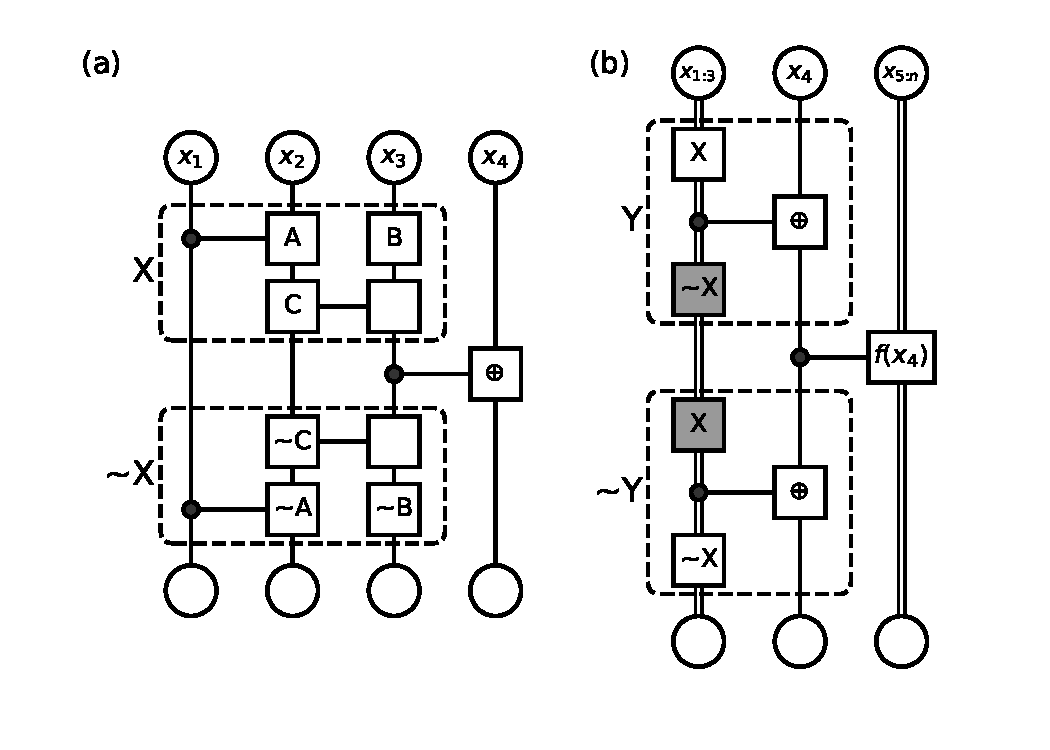
\includegraphics[width=\columnwidth,trim={0 1cm 0 0cm},clip]{images/fig6.pdf}}
    \caption{Data oriented computational graph that shows the compute-copy-uncompute paradigm. Circles connected by vertical lines are variables, where double lines represents multiple variables. Boxes and dots connected by parallel lines are operations. A dot on a line represents a control parameter while a box represents a mutable parameter.
    }\label{fig:ccu}
\end{figure}

Knowing the contents in the memory when deallocating is not easy. Hence Charles H. Bennett introduced the famous compute-copy-uncompute paradigm~\cite{Bennett1973}.
In order to show how reversible memory manage works, we introduce the memory oriented computational graph, as shown in \Fig{fig:ccu}.
Notations are highly inspired by quantum circuit representations. A vertical line is a variable, and it can be used by multiple operations. Hence it is a hypergraph rather than a simple graph like DAG. When a variable is used by a function, depending on whether its value is changed, we put a box or a dot at the cross.
Let us consider the example program shown in panel (a). The subprogram in dashed box \texttt{X} is executed on space $x_{1\colon3}$ to compute the desired result, which we call the computing stage. In the copying stage, the content in $x_3$ is read out to a pre-emptied memory $x_4$ through addition operation $\oplus$, and this is the piece of information that we care.
Since this copy operation does not change contents of $x_{1\colon3}$, we can use the inverse operation \texttt{$\sim$X} to undo all the changes to these registers. If a variable in $x_{1\colon3}$ is initialized as a known value like $0$, now it can be deallocated since its value is known again.
If this subroutine of generating $x_4$ is used in another program as shown in \Fig{fig:ccu} (b), $x_4$ can be uncomputed by the reversing the whole subroutine in panel (a).
The interesting fact is, both $X$ and $\sim X$ are executed twice in this program, which looks like unnecessary. We can, of cause cancel a pair of $X$ and $\sim X$ (the gray boxes). By doing this, we are not allowed to deallocate the memory $x_{1\colon3}$ during computing $f(x_4)$, i.e., additional space is required. The tradeoff between space and time will be discussed in detail in \Sec{sec:timespace}.

\subsubsection{Control flows}
The reversible \texttt{if} statement is shown in \Fig{fig:controlflow} (a). It contains a precondition and a postcondition. The precondition decides which branch to enter in the forward execution, while the postcondition decides which branch to enter in the backward execution. After executing the specific branch, the program checks the consistency between precondition and postcondition to make sure they are consistent.
The reversible \texttt{while} statement is shown in \Fig{fig:controlflow} (b). It also has both precondition and postcondition. Before executing the condition expressions, the program preassumes the postcondition is false.
After each iteration, the program asserts the postcondition to be true. In the reverse pass, we exchange the precondition and postcondition.
The reversible \texttt{for} statement is similar to irreversible ones except after executing the loop, and the program checks the values of these variables to make sure they are not changed. In the reverse pass, we exchange \texttt{start} and \texttt{stop} and inverse the sign of \texttt{step}.
\begin{figure}
    \centerline{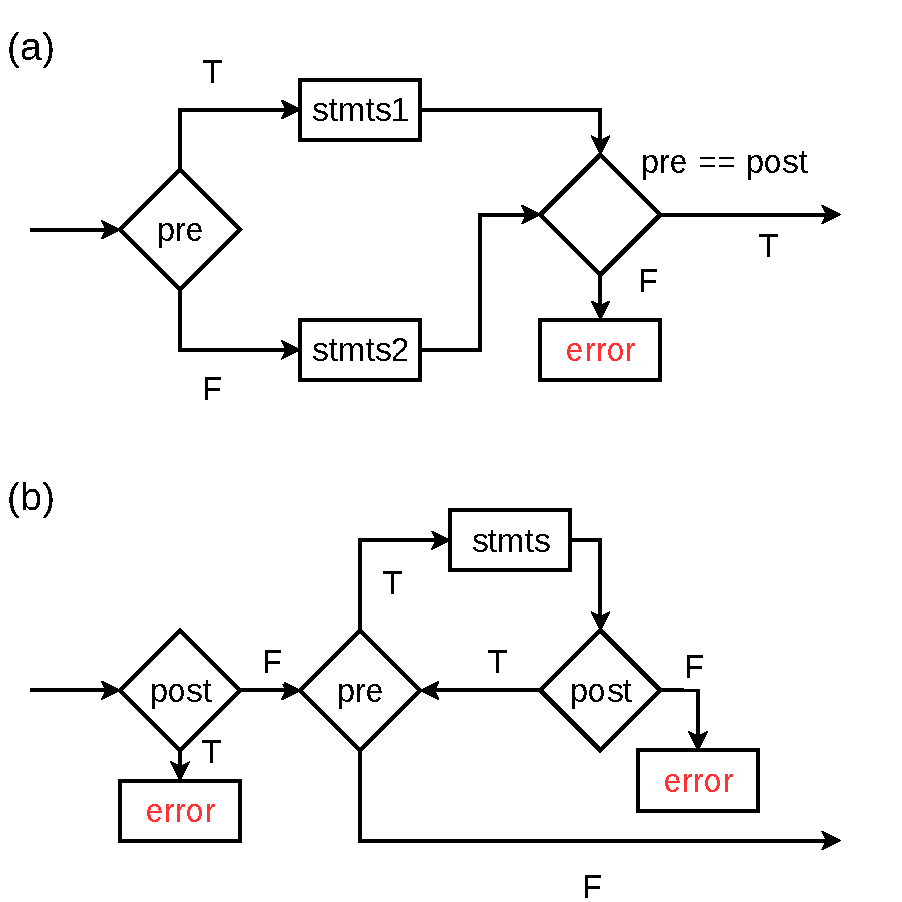
\includegraphics[width=0.8\columnwidth,trim={0 0cm 0 0cm},clip]{images/controlflow.pdf}}
    \caption{Flow chart for reversible (a) \texttt{if} statement and (b) \texttt{while} statement. ``stmts'', ``stmts1'' and ``stmts2'' are statements, statements in true branch and statements in false branch respectively. ``pre'' and ``post'' are precondition and postconditions respectively.}\label{fig:controlflow}
\end{figure}

\subsubsection{Arithmetic instructions}
Every arithmetic instruction has a unique inverse that can undo the changes.
For logical operations, we have \texttt{y $\veebar$= f(args...)} self reversible.
For other arithmetic operations, we regard \texttt{y += f(args...)} and \texttt{y -= f(args...)} are reversible to each other. Here \texttt{f} can be \texttt{identity}, \texttt{*}, \texttt{/} and \texttt{\^} et. al.
Besides the above two types of operations, \texttt{SWAP} operation that exchanges the contents in two memory spaces are also widely used in reversible computing systems.
Here, it is worth noticing that \texttt{+=} and \texttt{-=} are not precisely reversible to each other because floating-point number operations have the rounding error. For applications sensitive to rounding errors, we should consider using other number systems, which will be discussed in \Sec{sec:hardware}

\subsection{NiLang's Reversible IR}
In the last subsection, we have reviewed the basic building blocks of a typical reversible language. In order to insert the code of obtaining gradients into the reversed program, the reversible language design should have related abstraction power.
It can be achieved by utilizing the multiple-dispatch of Julia.
We can wrap a number with a particular type with a gradient field called \texttt{GVar} and dispatch it to instructions that update gradient fields for it.
Similar design is called \texttt{Dual} number in the tangent mode AD package ForwardDiff~\cite{Revels2016}.

The main feature of NiLang is contained in a single macro \texttt{@i} that compiles a reversible function.
The allowed statements in this eDSL are shown in \App{app:grammar}.
The following is a minimal example of compiling a NiLang function to native Julia function.

\begin{minipage}{.44\textwidth}
\begin{lstlisting}
julia> using NiLangCore, MacroTools

julia> macroexpand(Main, :(@i function f(x, y)
           SWAP(x, y)
       end)) |> MacroTools.prettify
quote
    $(Expr(:meta, :doc))
    function $(Expr(:where, :(f(x, y))))
        gaur = SWAP(x, y)
        x = (NiLangCore.wrap_tuple(gaur))[1]
        y = (NiLangCore.wrap_tuple(gaur))[2]
        return (x, y)
    end
    if typeof(f) != typeof(~f)
        function $(Expr(:where, :((  #$ TODO: remove this comment
                    mongoose::typeof(~f))(x, y))))
            mandrill = (~SWAP)(x, y)
            x = (NiLangCore.wrap_tuple(mandrill))[1]
            y = (NiLangCore.wrap_tuple(mandrill))[2]
            return (x, y)
        end
    end
    if !(NiLangCore._hasmethod1(
                NiLangCore.isreversible, typeof(f)))
        NiLangCore.isreversible(::typeof(f)) = true
    end
end
\end{lstlisting}
\end{minipage}

Macro \texttt{@i} generates three functions \texttt{f}, \texttt{$\sim$f} and \texttt{NiLangCore.isreversible}. \texttt{f} and \texttt{$\sim$f} are a pair of functions that are reversbile to each other, where \texttt{$\sim$f} is an callable of type \texttt{Inv\{typeof(f)\}}.
In the body of \texttt{f}, \texttt{NiLangCore.wrap\_tuple} is used to unify output data types to tuples.
The outputs of \texttt{SWAP} are assigned back to its input variables. In other words, it simulates a function that modifies inputs inplace.
At the end of this function, this macro attaches a return statement that returns all input variables.
Finally, it defines \texttt{NiLangCore.isreversible} for \texttt{f} to mark it as reversible.

To understand the design of reversibility, we first introduce a reversible IR that plays a central role in NiLang.
In this IR, a statement can be an instruction, a function call, a control flow, a memory allocation/deallocation, or the inverse statement ``$\sim$''.
Any statement is this IR has a unique inverse, as shown in \Tbl{tbl:revstatements}.

\begin{table}[h!]\centering
\begin{minipage}{\columnwidth}
\ra{1.3}
    \scalebox{1.0}{
        \begin{tabularx}{\textwidth}{X X}\toprule
            \textbf{statement} & \textbf{inverse}\\
            \hline
            \texttt{<f>(<args>...)} & \texttt{($\sim$<f>)(<args>...)}\\
            \hline
            \texttt{<y> += <f>(<args>...)} & \texttt{<y> -= <f>(<args>...)}\\
            \hline
            \texttt{<y> .+= <f>.(<args>...)} & \texttt{<y> .-= <f>.(<args>...)}\\
            \hline
            \texttt{<y> $\veebar$= <f>(<args>...)} & \texttt{<y> $\veebar$= <f>(<args>...)}\\
            \hline
            \texttt{<y> .$\veebar$= <f>(<args>...)} & \texttt{<y> .$\veebar$= <f>(<args>...)}\\
            \hline
            \texttt{<a> $\leftarrow$ <expr>} & \texttt{<a> $\rightarrow$ <expr>}\\
            \hline
            \texttt{(<T1> => <T2>)(<x>)} & \texttt{(<T2> => <T1>)(<x>)}\\
            \hline
            \texttt{begin}\newline \texttt{$\cquad$<stmts>}\newline \texttt{end} & \texttt{begin}\newline \texttt{$\cquad$ $\sim$(<stmts>)}\newline \texttt{end}\\
            \hline
            \texttt{if (<pre>, <post>)}\linebreak \texttt{$\cquad$<stmts1>}\newline \texttt{else}\newline \texttt{$\cquad$<stmts2>}\newline \texttt{end} & \texttt{if (<post>, <pre>)}\newline \texttt{$\cquad$$\sim$(<stmts1>)}\newline \texttt{else}\newline \texttt{$\cquad$ $\sim$(<stmts2>)}\newline \texttt{end}\\
            \hline
            \texttt{while (<pre>, <post>)}\newline \texttt{$\cquad$<stmts>} \newline \texttt{end} & \texttt{while (<post>, <pre>)}\newline $\cquad$  \texttt{$\sim$(<stmts>)}\newline \texttt{end}\\
            \hline
            \texttt{for <i>=<m>:<s>:<n>}\newline $\cquad$\texttt{<stmts>}\newline \texttt{end} & \texttt{for <i>=<m>:-<s>:<n>}\newline $\cquad$ \texttt{$\sim$(<stmts>)}\newline \texttt{end}\\
            \hline
            \texttt{@safe <expr>} & \texttt{@safe <expr>}\\
            \bottomrule
        \end{tabularx}
    }
    \caption{A collection of reversible statements, where left side and right side are reversible to each other.
    ``.'' is the symbol for broadcasting magic in Julia,
    ``$\sim$'' is the symbol for reversing a statement or a function.
    \texttt{<pre>} stands for precondition, 
    \texttt{<post>} stands for postcondition,
    \texttt{<args>...} stands for the argument list of a function,
    \texttt{<stmts>} stands for statement,
    \texttt{<exprs>} stands for expression,
    \texttt{<T1>} and \texttt{<T2>} stand for types.
}\label{tbl:revstatements},
\end{minipage}
\end{table}

%For example, an instruction \texttt{y $\mathrel{+}=$ f(args...)} is interpreted as a Julia function call \texttt{PlusEq(f)(y, args...)} or \texttt{$\oplus$(f)(y, args...)} as a shorthand.
%Here, the ``!'' after a variable is used as a convension to indicate that a variable is changed after the call of an instruction or function.
%The detailed specification of instructions is listed in \App{app:instr}. The function call is same as the host language, except every function \texttt{f} has a \texttt{$\sim$f} that binded to an object of type \texttt{Inv\{typeof(f)\}}. \texttt{$\sim$f} invokes the compiled inverse functions of \texttt{f}.

%This design allows users putting additional postcondition in control flows to help reverse the program.
%A postcondition is a boolean expression that being evaluated after the body expressions being executed.
``\texttt{$\leftarrow$}'' and ``\texttt{$\rightarrow$}'' are symbols for memory allocation and deallocation, one can input them by typing ``$\backslash$leftarrow'' and ``$\backslash$rightarrow'' respectively followed by a Tab key in a Julia editor or REPL.
``\texttt{begin <stmts> end}'' is the block statement in Julia, it represents a code block.
It can be inverted by reversing the order as well as each element in it.
A \texttt{if} or \texttt{while} statement is similar to its native Julia counterpart, except the conditional expression in statements is a tuple of precondition and postcondition.
%\texttt{<a> $\leftarrow$ <expr>} binds variable \texttt{<a>} to an initial value specified by \texttt{<expr>}. Its inverse \texttt{<a> $\rightarrow$ <expr>} deallocates the variable \texttt{<a>}. Before deallocating the variable, the program checks that the its value is the same as the value of \texttt{<expr>}, otherwise throws an \texttt{InvertibilityError}.
%A function call in NiLang supports Julia's broadcasting magic, a function defined on scalars can be broadcasted to vectors by adding a ``.'' after the function call.
%\texttt{$\rightarrow$} will be added automatically.
    %The additional check underlines the difference between the irreversible assign statement and reversible ancilla statement.
Finally, the macro \texttt{@safe} allows users to use external statements that do not break reversibility.
For example, one can use \texttt{@safe @show <var>} for debugging.

\subsection{Compiling}
The compilation of a reversible function contains three stages.

\begin{figure}[h]
    \centerline{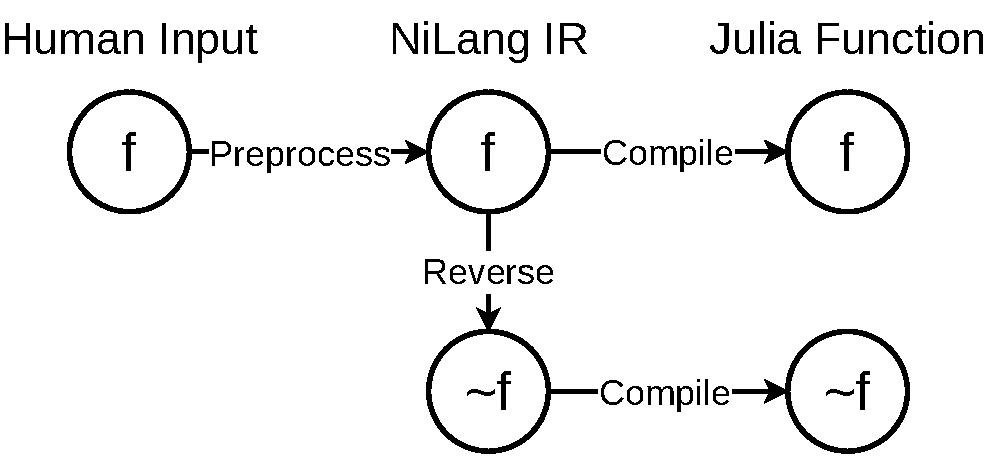
\includegraphics[width=0.7\columnwidth,trim={0cm 0cm 0 0cm},clip]{images/compiling.pdf}}
    %\caption{Three compiling stages of NiLang.}\label{fig:compiling}
\end{figure}

The first stage pre-processes human inputs to a reversible IR.
The preprocessor expands the symbol ``\texttt{$\sim$}'' in the postcondition field of \texttt{if} statement by copying the precondition, adds missing ancilla ``$\leftarrow$'' statements to ensure ``\texttt{$\leftarrow$}'' and ``\texttt{$\rightarrow$}'' appear in pairs inside a function, a \texttt{while} statement or a \texttt{for} statement, and expands the uncomputing macro \texttt{$\sim$@routine}.
Since the compute-copy-uncompute paradigm is extensively used in reversible programming to uncompute ancillas, one can use \texttt{@routine <stmt>} statement to record a statement, and \texttt{$\sim$@routine} to insert \texttt{$\sim$<stmt>} for uncomputing.
The following example pre-processes an \texttt{if} statement to the reversible IR.

\begin{minipage}{.44\textwidth}
\begin{lstlisting}
julia> using NiLangCore, MacroTools

julia> NiLangCore.precom_ex(
       :(if (x > 3, ~)
            @routine z += x * y
            ~@routine
       end), NiLangCore.PreInfo()
       ) |> MacroTools.prettify
:(if (x > 3, x > 3)
      z += x * y
      z -= x * y
  else
  end)
\end{lstlisting}
\end{minipage}

In this example, since the precondition ``\texttt{x > 3}'' is not change after execution of the specific branch, we omit the postcondition by putting a ``$\sim$'' in this field. ``\texttt{@routine}'' records a statement, the statement can also be a ``\texttt{begin <stmts> end}'' block as a sequence of statements.

The second stage generates the reversed code according to table \Tbl{tbl:revstatements}. For example,

\begin{minipage}{.44\textwidth}
\begin{lstlisting}
julia> NiLangCore.dual_ex(
       :(if (pre, post)
           z += x * y
       else
           z += x / y
       end)
       ) |> MacroTools.prettify
:(if (post, pre)
      z -= x * y
  else
      z -= x / y
  end)
\end{lstlisting}
\end{minipage}

The third stage is translating this IR and its inverse to native Julia code. It explains all functions as inplace and inserts codes about reversibility check. At the end of a function definition, it attaches a return statement that returns all input arguments.
After this, the function is ready to execute on the host language.
The following example shows how an \texttt{if} statement is transformed in this stage.

\begin{minipage}{.44\textwidth}
\begin{lstlisting}
julia> NiLangCore.compile_ex(
       :(if (pre, post)
           z += x * y
       else
           z += x / y
       end), NiLangCore.CompileInfo()
       ) |> MacroTools.prettify
quote
    bat = pre
    if bat
        @assignback (PlusEq(*))(z, x, y)
    else
        @assignback (PlusEq(/))(z, x, y)
    end
    @invcheck post bat
end
\end{lstlisting}
\end{minipage}

The compiler translates the instruction according to \Tbl{tbl:interp} and adds \texttt{@assignback} before each instruction and function call statement. The macro \texttt{@assignback} assigns the output of a function back to the arguments of that function. \texttt{@invcheck post bat} checks the consistency between preconditions and postconditions to ensure reversibility. This statement will throw an \texttt{InvertibilityError} error if target variables \texttt{bat} and \texttt{post} are not ``equal'' to each other up to a certian torlerance.

\subsection{Types and Dataviews}
So far, the language design is not too different from a traditional reversible language. To implement the adjoint mode AD, we introduce types and dataviews.
The type used in the reversible context is just a standard Julia type with an additional requirement of having reversible constructors.
The inverse of a constructor is called a ``destructor'', which unpacks data and deallocates derived fields.
A reversible constructor is implemented by reinterpreting the \texttt{new} function in Julia.
Let us consider the following statement.

\begin{minipage}{.44\textwidth}
\begin{lstlisting}
    x ← new{TX, TG}(x, g)
\end{lstlisting}
\end{minipage}

The above statement is similar to allocating an ancilla, except it deallocates \texttt{g} directly at the same time.
Doing this is proper because \texttt{new} is special that its output keeps all information of its arguments. All input variables that do not appear in the output can be discarded safely. Its inverse is

\begin{minipage}{.44\textwidth}
\begin{lstlisting}
    x → new{TX, TG}(x, g)
\end{lstlisting}
\end{minipage}

It unpacks structure \texttt{x} and assigns fields to corresponding variables in the argument list.
The following example shows a non-complete definition of the reversible type \texttt{GVar}.

\begin{minipage}{.44\textwidth}
\begin{lstlisting}
julia> using NiLangCore

julia> @i struct GVar{T,GT} <: IWrapper{T}
           x::T
           g::GT
           function GVar{T,GT}(x::T, g::GT) where
                                       {T,GT}
               new{T,GT}(x, g)
           end
           function GVar(x::T, g::GT) where {T,GT}
               new{T,GT}(x, g)
           end
           @i function GVar(x::T) where T
               g ← zero(x)
               x ← new{T,T}(x, g)
           end
           @i function GVar(x::AbstractArray)
               GVar.(x)
           end
       end

julia> GVar(0.5)
GVar{Float64,Float64}(0.5, 0.0)

julia> (~GVar)(GVar(0.5))
0.5

julia> (~GVar)(GVar([0.5, 0.6]))
2-element Array{Float64,1}:
 0.5
 0.6
\end{lstlisting}
\end{minipage}

\texttt{GVar} has two fields that correspond to the value and gradient of a variable.
Here, we put \texttt{@i} macro before both \texttt{struct} and \texttt{function} statements.
The ones before functions generate forward and backward functions, while the one before \texttt{struct} moves \texttt{$\sim$GVar} functions to the outside of the type definition. Otherwise, the inverse function will be ignored by Julia compiler.

Since an operation changes data inplace in NiLang, hence a field of an immutable instance should also be `` modifiable''.
Let us first consider the following example.

\begin{minipage}{.44\textwidth}
\begin{lstlisting}
julia> arr = [GVar(3.0), GVar(1.0)]
2-element Array{GVar{Float64,Float64},1}:
 GVar{Float64,Float64}(3.0, 0.0)
 GVar{Float64,Float64}(1.0, 0.0)

julia> x, y = 1.0, 2.0
(1.0, 2.0)

julia> @instr -arr[2].g += x * y
2.0

julia> arr
2-element Array{GVar{Float64,Float64},1}:
 GVar{Float64,Float64}(3.0, 0.0) 
 GVar{Float64,Float64}(1.0, -2.0)
\end{lstlisting}
\end{minipage}

In Julia language, the assign statement above will throw a syntax error because the function call ``\texttt{-}'' can not be assigned, and \texttt{GVar} is an immutable type.
In NiLang, we use the macro \texttt{@assignback} to modify an immutable data directly. It translates the above statement to

\begin{minipage}{.44\textwidth}
\begin{lstlisting}[numberstyle=\scriptsize\color{gray},numbers=left,numbersep=8pt]
res = (PlusEq(*))(-arr[2].g, x, y)
arr[2] = chfield(arr[2], Val(:g),
    chfield(arr[2].g, -, res[1]))
x = res[2]
y = res[3]
\end{lstlisting}
\end{minipage}

The first line \texttt{PlusEq(*)(-arr[3].g, x, y)} computes the output as a tuple of length $3$.
At lines 2-3, \texttt{chfield(x, Val\{:g\}, val)} modifies the \texttt{g} field of \texttt{x} and \texttt{chfield(x, -, res[1])} returns \texttt{-res[1]}. Here, modifying a field requires the default constructor of a type not overwritten.
The assignments in lines 4 and 5 are straightforward.
We call a bijection of a field of an object a ``dataview'' of this object, and it is directly modifiable in NiLang.
The definition of dataview can be found in \App{app:grammar}.

\section{Reversible automatic differentiation}\label{sec:bp}

Local Jacobians and Hessians for basic instructions used in this section could be found in \App{app:jacobians}.

\subsection{First order gradient}\label{sec:jacobian}
Consider a computation $\vx^{i-1} = f_{i}^{-1}(\vx^{i})$ in a reversed program, the Jacobians can be propagated in the reversed direction like
\begin{align}
    \begin{split}
        J^{\out}_{\out'} &= \delta_{\out,\out'},\\
        J^{\out}_{\vx^{i-1}} &= J^{\out}_{\vx^i} J^{\vx^i}_{\vx^{i-1}},
    \end{split}\label{eq:jacobian}
\end{align}
where $\out$ represents the outputs of the program. In adjoint mode AD, it is a scalar.
$J^{\out}_{\vx^i} \equiv \frac{\partial \out}{\partial \vx^i}$ is the Jacobian to be propagated, and $J^{\vx^i}_{\vx^{i-1}}$ is the local Jacobian matrix. Einstein's notation~\cite{Einsum} is used here so that the duplicated index $\vx^{i}$ in the second line is summed over.
\Eq{eq:jacobian} can be rewritten in the diagram of tensor networks~\cite{Orus2014} as shown in \Fig{fig:ad}.
\begin{figure}
    \centerline{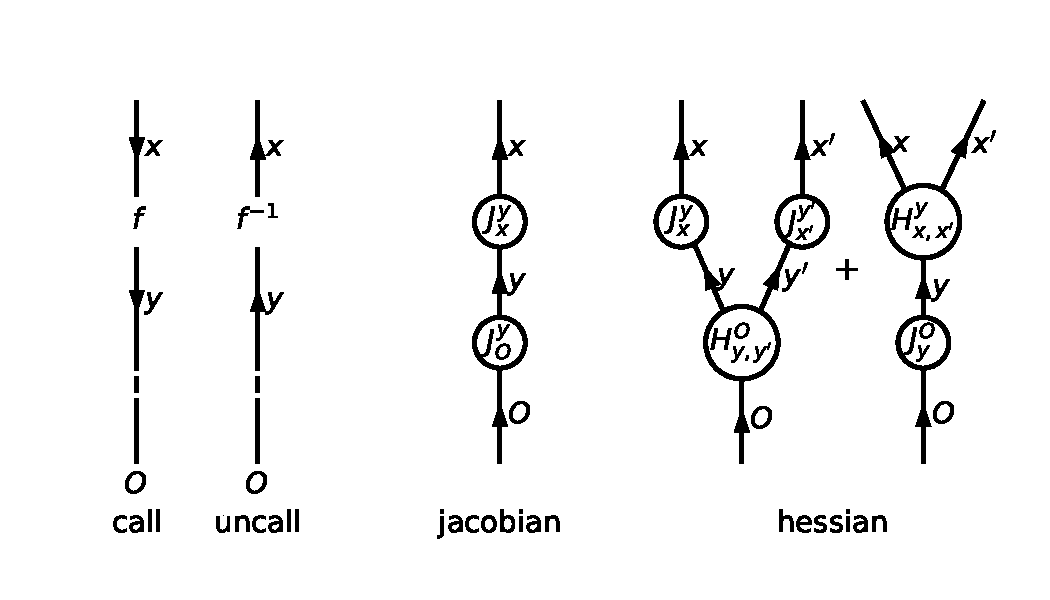
\includegraphics[width=0.95\columnwidth,trim={0.5cm 1cm 0 1cm},clip]{images/ad.pdf}}
    \caption{Computational processes in the tensor network diagram, a big circle with three legs represent a Hessian, a small circle with two legs represents a Jacobian. Dangling edges and connected edges stand for unpaired and paired labels, respectively in Einstein's notation. From left to right, the diagrams represent computing, uncomputing, Jacobian propagation, and Hessian propagation.}\label{fig:ad}
\end{figure}
The algorithm to compute the adjoint mode AD can be summarized as follows.

\begin{algorithm}[H]
    \KwResult{\grad.($\vx$)}
    let \texttt{iloss} be the index of the loss in $\vx$\\
    $\vx \leftarrow f(\vx)$\\
    \For{k = 1:length($\vx$)}{
        $\vx_k \leftarrow$ \texttt{GVar}($\vx_k$, $\delta_{k, {\rm iloss}}$)\\
    }
    $\vx \leftarrow f^{-1}(\vx)$
    \caption{Reversible programming AD}\label{alg:ad}
\end{algorithm}

We first compute the results with the forward pass $f(x)$.
Then we wrap each output with a gradient field. The gradient field is initialized to 1 if the variable is the loss else 0. Then we run the backward pass $f^{-1}(x)$ to update the gradient fields of variables.
The gradients can be accessed using the $\grad$ dataview of output variables.
%Its inverse \texttt{$\sim$GVar} deallocates the gradient field safely and returns its value field.  Here, "safely" means before deallocation, the program will check the gradient field to make sure its value is restored to $0$.
%When an instruction \texttt{instruct} meets a \texttt{GVar}, besides computing its value field $\vvalue(\vy) = \texttt{instruct}(\vvalue(\vx))$, it also updates the gradient field $\grad(\vy) = \left[J^{\vy}_{\vx}\right]^{-1} \grad(\vx)$, where $\left[J^{\vy}_{\vx}\right]^{-1}$ is the Jacobian of $\texttt{instruct}^{-1}$. One can define this gradient function on either \texttt{instruct} or \texttt{instruct${}^{-1}$}.
The computation of gradients is implemented with multiple-dispatch. That is, when an instruction meets a \texttt{GVar} instance, it calls a different routine. For example, the backward rules for instructions \texttt{$\oplus(*)$} and \texttt{$\ominus(*)$} can be defined by overloading \textbf{either} of them as following.

\begin{minipage}{.44\textwidth}
\begin{lstlisting}[mathescape=true]
@i function ⊖(*)(out!::GVar, x::GVar, y::GVar)
    value(out!) -= value(x) * value(y)
    grad(x) += grad(out!) * value(y)
    grad(y) += value(x) * grad(out!)
end
\end{lstlisting}
\end{minipage}

%Here, we adopt the convention that only variables ended with \texttt{!} will be changed after the function call.
%This backward rule has been included in NiLang, one can check the gradients by typing in a Julia REPL
%If one defines the backward rule on \texttt{instruct}, the compiler will generate the backward rule for its inverse \texttt{instruct${}^{-1}$} as the inverse function. This is doable 
We use the backward rule defined on $\ominus(*)$ to backpropagate the function $\oplus(*)$.
Since taking inverse and computing gradients commute to each other~\cite{Mcinerney2015}, the compiler also binds the backward function on $\oplus(*)$ automatically.
%When gradients are not used anymore, the reversible way to deallocate gradients is uncomputing the whole process of obtaining them.
%, which increases the hyrachy by 1. Whenever the hyrachy increase by 1, the computational overhead doubles comparing with its irreversible counter part.
One can check the correctness of this definition as follows.

\begin{minipage}{.44\textwidth}
\begin{lstlisting}[mathescape=true]
julia> using NiLang, NiLang.AD

julia> a, b, y = GVar(0.5), GVar(0.6), GVar(0.9)
(GVar(0.5, 0.0), GVar(0.6, 0.0), GVar(0.9, 0.0))

julia> @instr grad(y) += identity(1.0)

julia> @instr y += a * b
GVar(0.6, -0.5)

julia> a, b, y
(GVar(0.5, -0.6), GVar(0.6, -0.5), GVar(1.2, 1.0))

julia> @instr y -= a * b
GVar(0.6, 0.0)

julia> a, b, y
(GVar(0.5, 0.0), GVar(0.6, 0.0), GVar(0.899999, 1.0))
\end{lstlisting}
\end{minipage}

Here, since $J(\ominus(*)) = J(\oplus(*))^{-1}$, consecutively applying them will restore the gradient fields of all variables.
The overhead of using \texttt{GVar} type is negligible thanks to Julia's multiple-dispatch and type inference.


\subsection{Second-order gradient}
Second-order gradients can be obtained in three different approaches, forward differentiating the adjoint program, adjoint differentiating the adjoint program, and Hessian propagation.
\subsubsection{Forward differentiating the adjoint program}\label{sec:dualhessian}
Combining the adjoint program in NiLang with dual-numbers is a simple yet efficient way to obtain Hessians.
By wrapping the elementary type with \texttt{Dual} defined in package ForwardDiff~\cite{Revels2016} and throwing it into the gradient program defined in NiLang,
one obtains one row/column of the Hessian matrix straightforward.
We will show an example of using forward differentiating in Newton's trust region optimization in \Sec{sec:graph}.

\subsubsection{Adjoint differentiating the adjoint program}\label{sec:simplehessian}
Back propagating first-order gradients is also widely used to obtain the second-order gradients. Suppose the function space is closed under gradient operation, one can obtain higher-order gradients by recursively differentiating lower-order gradient functions without defining new backward rules. An example is shown in \App{app:hessian}.

\subsubsection{Hessian propagation}\label{sec:taylor}
It is also possible to back-propagate Hessians directly~\cite{Martens2012} using the relation
\begin{align}
    \begin{split}
        &H^{\out}_{\vx^{L'},\vx^{L''}} = \mathbf{0},\\
        &H^{\out}_{\vx^{i-1},\vx^{i-1'}} = J^{\vx^i}_{\vx^{i-1}} H^{\out}_{\vx^i, \vx^{i'}} J^{\vx^{i'}}_{\vx^{i-1'}} + J^{\out}_{\vx^i} H^{\vx^i}_{\vx^{i-1}, \vx^{i-1'}}.
    \end{split}
\end{align}
Here, the Hessian is represented as a tensor $H^{\out}_{\vx^{i-1},\vx^{i-1'}}$ of rank three.
In the tensor network diagram, the above equation can be represented as the right panel of \Fig{fig:ad}.
The advantage of using Hessian propagation is that it can be generalized to Taylor propagation in the future.
Concerning the order of gradients, Taylor propagation is exponentially more efficient in obtaining higher-order gradients than differentiating lower-order gradients recursively. %The later requires traversing the computational graph repeatedly.
%In JAX~\cite{Bettencourt2019}, in order to support Taylor propagation, the propagation rules for part of primitives should be manually defined.
Comparing with operator overloading, source-to-source automatic differentiation has the advantage of having very limited primitives, exhausted support to Hessian propagation is possible.
An example to obtain Hessians is provided in \Sec{sec:bessel}.

\subsection{Gradient on ancilla problem}
In this section, we introduced an easily overlooked problem in our reversible AD framework.
An ancilla can sometimes carry a nonzero gradient when it is going to be deallocated. As a result, even if an ancilla can be uncomputed rigorously in the original program, its \texttt{GVar} wrapped version is not necessarily safely deallocated.
In NiLang, we drop the gradient field of ancillas instead of raising an error.
In the following, we justify our decision by proving the following theorem
\begin{theorem}
    Deallocating an ancilla with constant value field and nonzero gradient field does not harm the reversibility of a function.
\end{theorem}
\begin{proof}
    Consider a reversible function $\vx^i, b = f_i(\vx^{i-1}, a)$, where $a$ and $b$ are the input and output values of an ancilla.
    Since both $a$, $b$ are constants that are indenpedent of input $\vx^{i-1}$, we have
\begin{align}
    \frac{\partial b}{\partial \vx^{i-1}} = \mathbf{0}.
\end{align}
%Suppose in the backward pass, we discard the gradient field of $b$.
%So the question becomes does \texttt{grad(b)} have effect on the $\vx$?
Discarding gradients should not have any effect on the \texttt{value} fields of outputs.
    The key is to show $\texttt{grad(b)} \equiv \frac{\partial \vx^L}{\partial{b}}$ does appear in the \texttt{grad} fields of the output. It can be seen from the back-propagation rule 
\begin{equation}
    \frac{\partial \vx^L}{\partial \vx^{i-1}} = \frac{\partial \vx^L}{\partial \vx^i}\frac{\partial \vx^i}{\partial \vx^{i-1}} + \frac{\partial \vx^L}{\partial b}\frac{\partial b}{\partial \vx^{i-1}},
\end{equation}
where the second term with $\frac{\partial \vx^L}{\partial{b}}$ vanishes naturally.
\end{proof}

\section{Examples}\label{sec:example}

In this section, we introduce several examples.
We will discuss the first example, the first kind Bessel function, in most detail.
We compare the difference between the irreversible and reversible implementations of this function, as well as the difference between regular computational graph and memory oriented computational graph.
Then we show how to obtain first and second-order gradients automatically in the reversible AD framework.
We benchmark different source-to-source AD implementations of the Bessel function.
Then we show how to differentiate sparse matrix operations, unitary matrix multiplication, and QR decomposition.
Finally, we show how to solve the graph embedding problem variati

\subsection{The first kind Bessel function}\label{sec:bessel}
A Bessel function of the first kind of order $\nu$ can be computed using Taylor expansion
\begin{equation}
    J_\nu(z) = \sum\limits_{n=0}^{\infty} \frac{(z/2)^\nu}{\Gamma(k+1)\Gamma(k+\nu+1)} (-z^2/4)^{n}
\end{equation}
where $\Gamma(n) = (n-1)!$ is the Gamma function. One can compute the accumulated item iteratively as $s_n = -\frac{z^2}{4} s_{n-1}$. The irreversible implementation is

\begin{minipage}{.44\textwidth}
\begin{lstlisting}
function besselj(ν, z; atol=1e-8)
    k = 0
    s = (z/2)^ν / factorial(ν)
    out = s
    while abs(s) > atol
        k += 1
        s *= (-1) / k / (k+ν) * (z/2)^2
        out += s
    end
    out
end
\end{lstlisting}
\end{minipage}

This computational process could be diagrammatically represented as a DAG as show in \Fig{fig:cgraphs}(\subref{fig:computational-graph}).
In this diagram, the data is represented as an edge. It connects at most two nodes. One generates this data, and one consumes it.
A computational graph is more likely a mathematical expression, and it can not describe inplace functions or control flows conveniently because it does not have the notation for memory and loops.
%\begin{figure*}
    %\centerline{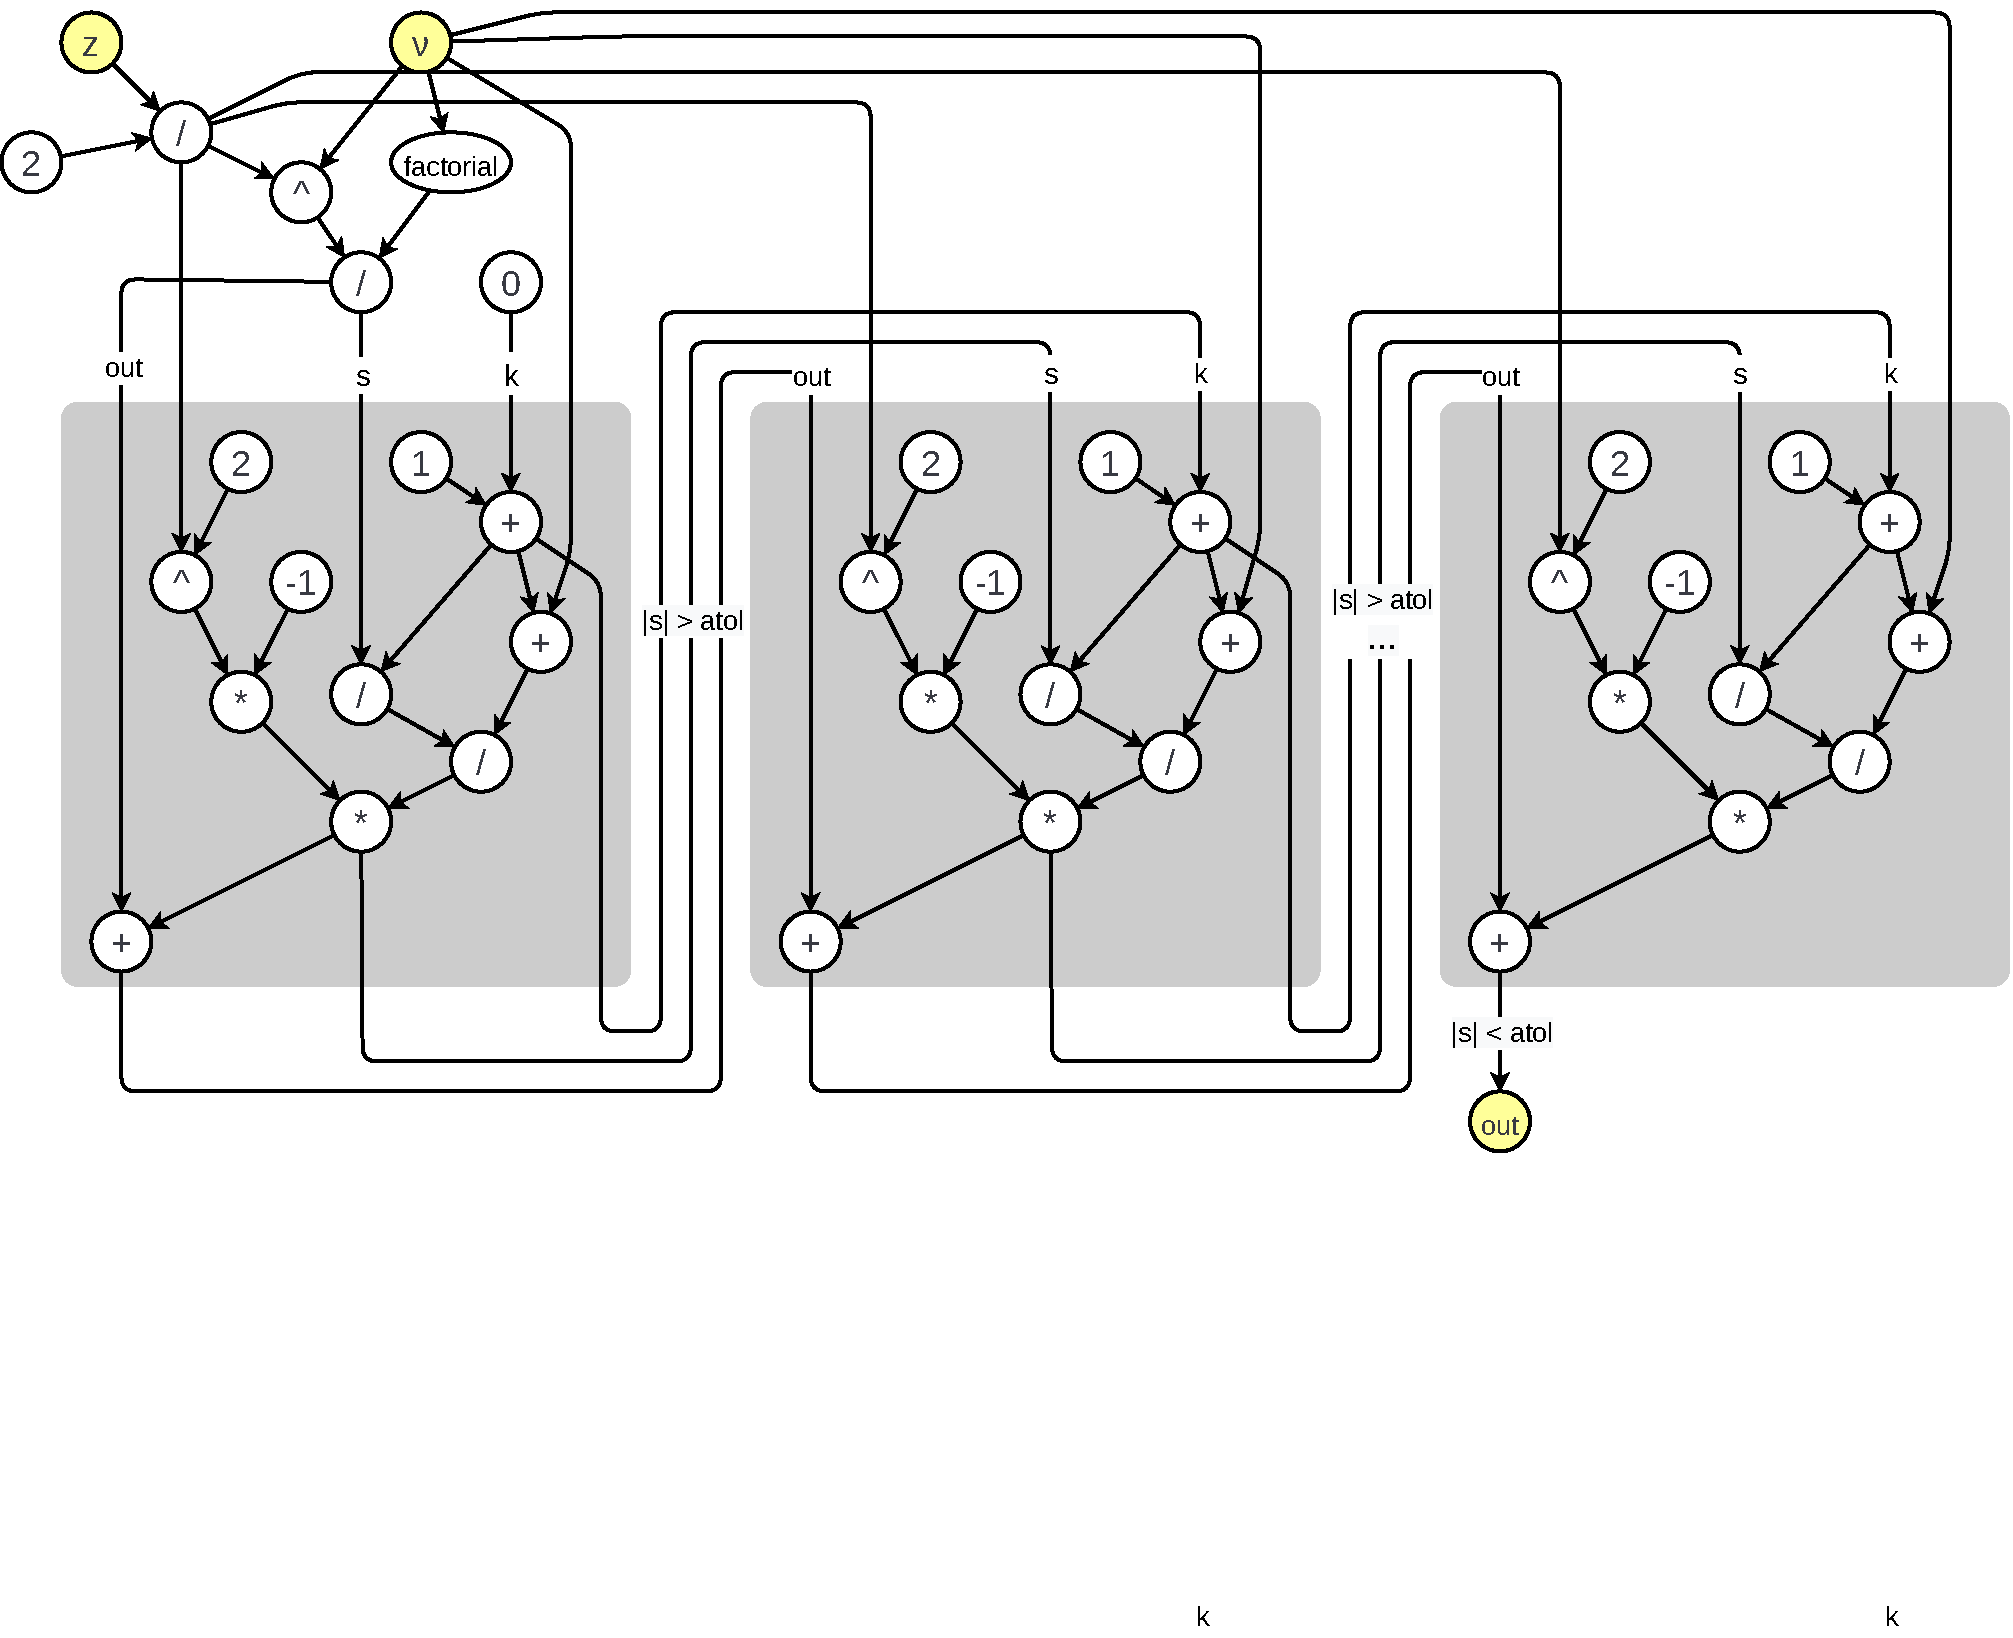
\includegraphics[width=0.8\textwidth,trim={0cm 6cm 0 0},clip]{images/computational_graph.pdf}}
    %\caption{Traditional computational graph for the reversible first kind Bessel function. Where a vertex (circle) is an operation and a directed edge is a variable. The gray region is the body of while loop.}\label{fig:computational-graph}
%\end{figure*}
\begin{figure*}[t!]
    \centering
    \begin{subfigure}[t]{0.53\textwidth}
        \centering
        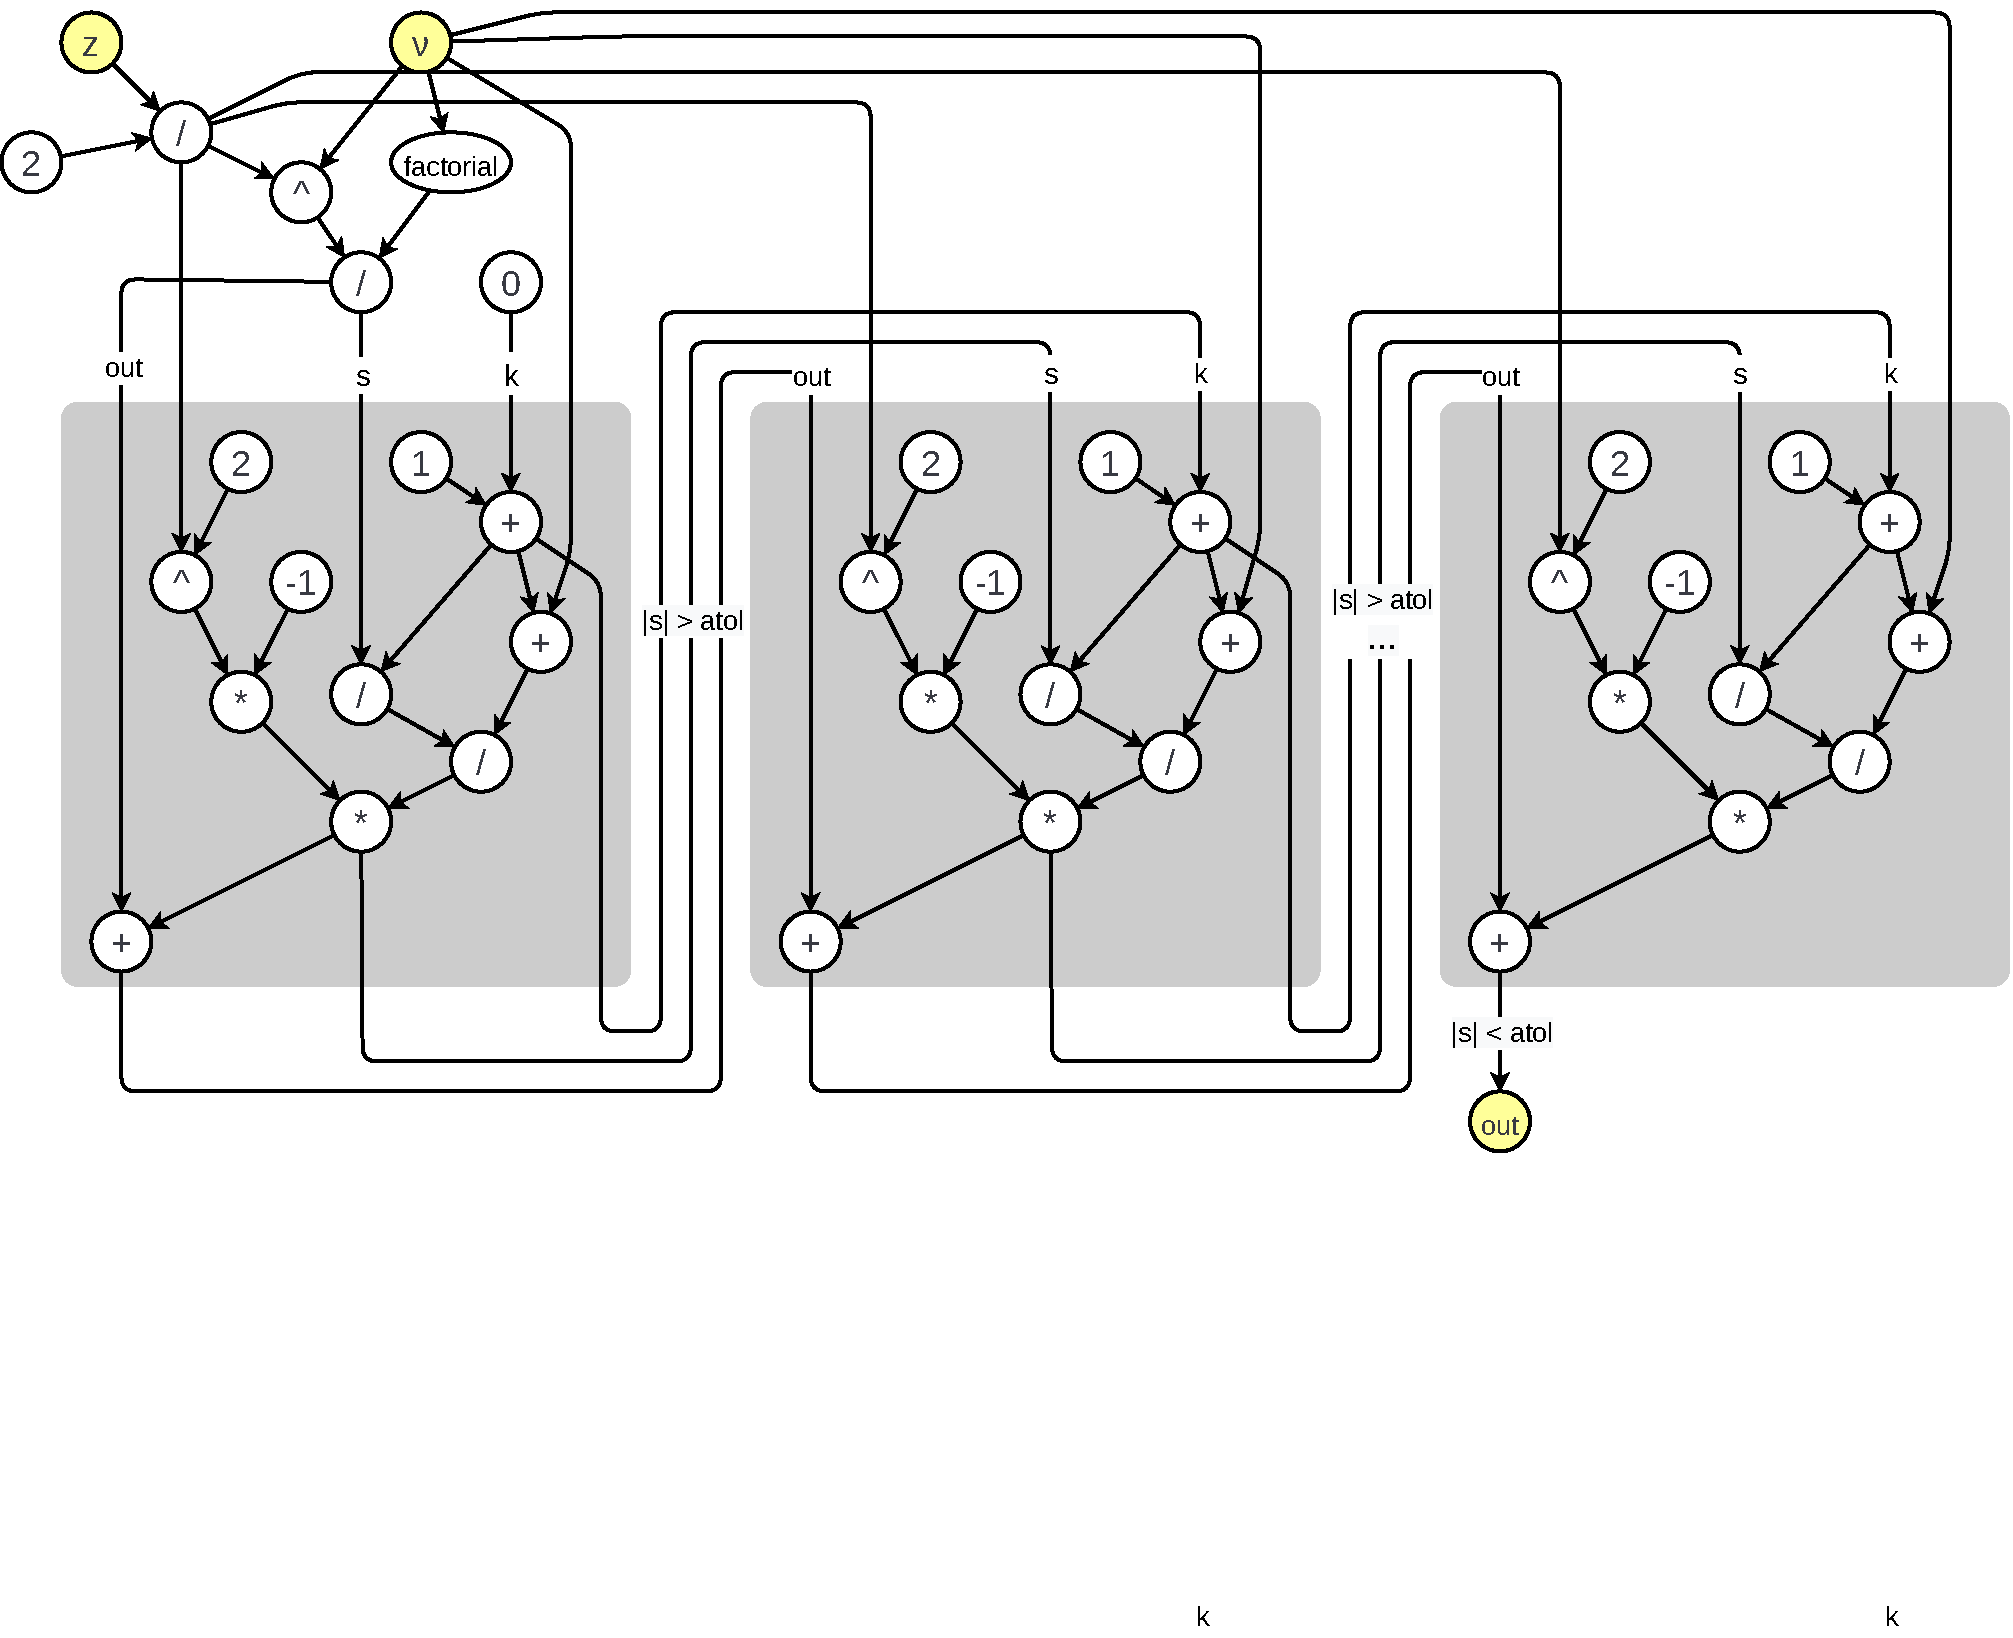
\includegraphics[width=\columnwidth,trim={0 4cm 0 0cm},clip]{images/computational_graph.pdf}
        \caption{Where a vertex (circle) is an operation, and a directed edge is a variable. The gray region is the body of the while loop. The while loop is unrolled.}\label{fig:computational-graph}
    \end{subfigure}%
    \begin{subfigure}[t]{0.47\textwidth}
        \centering
        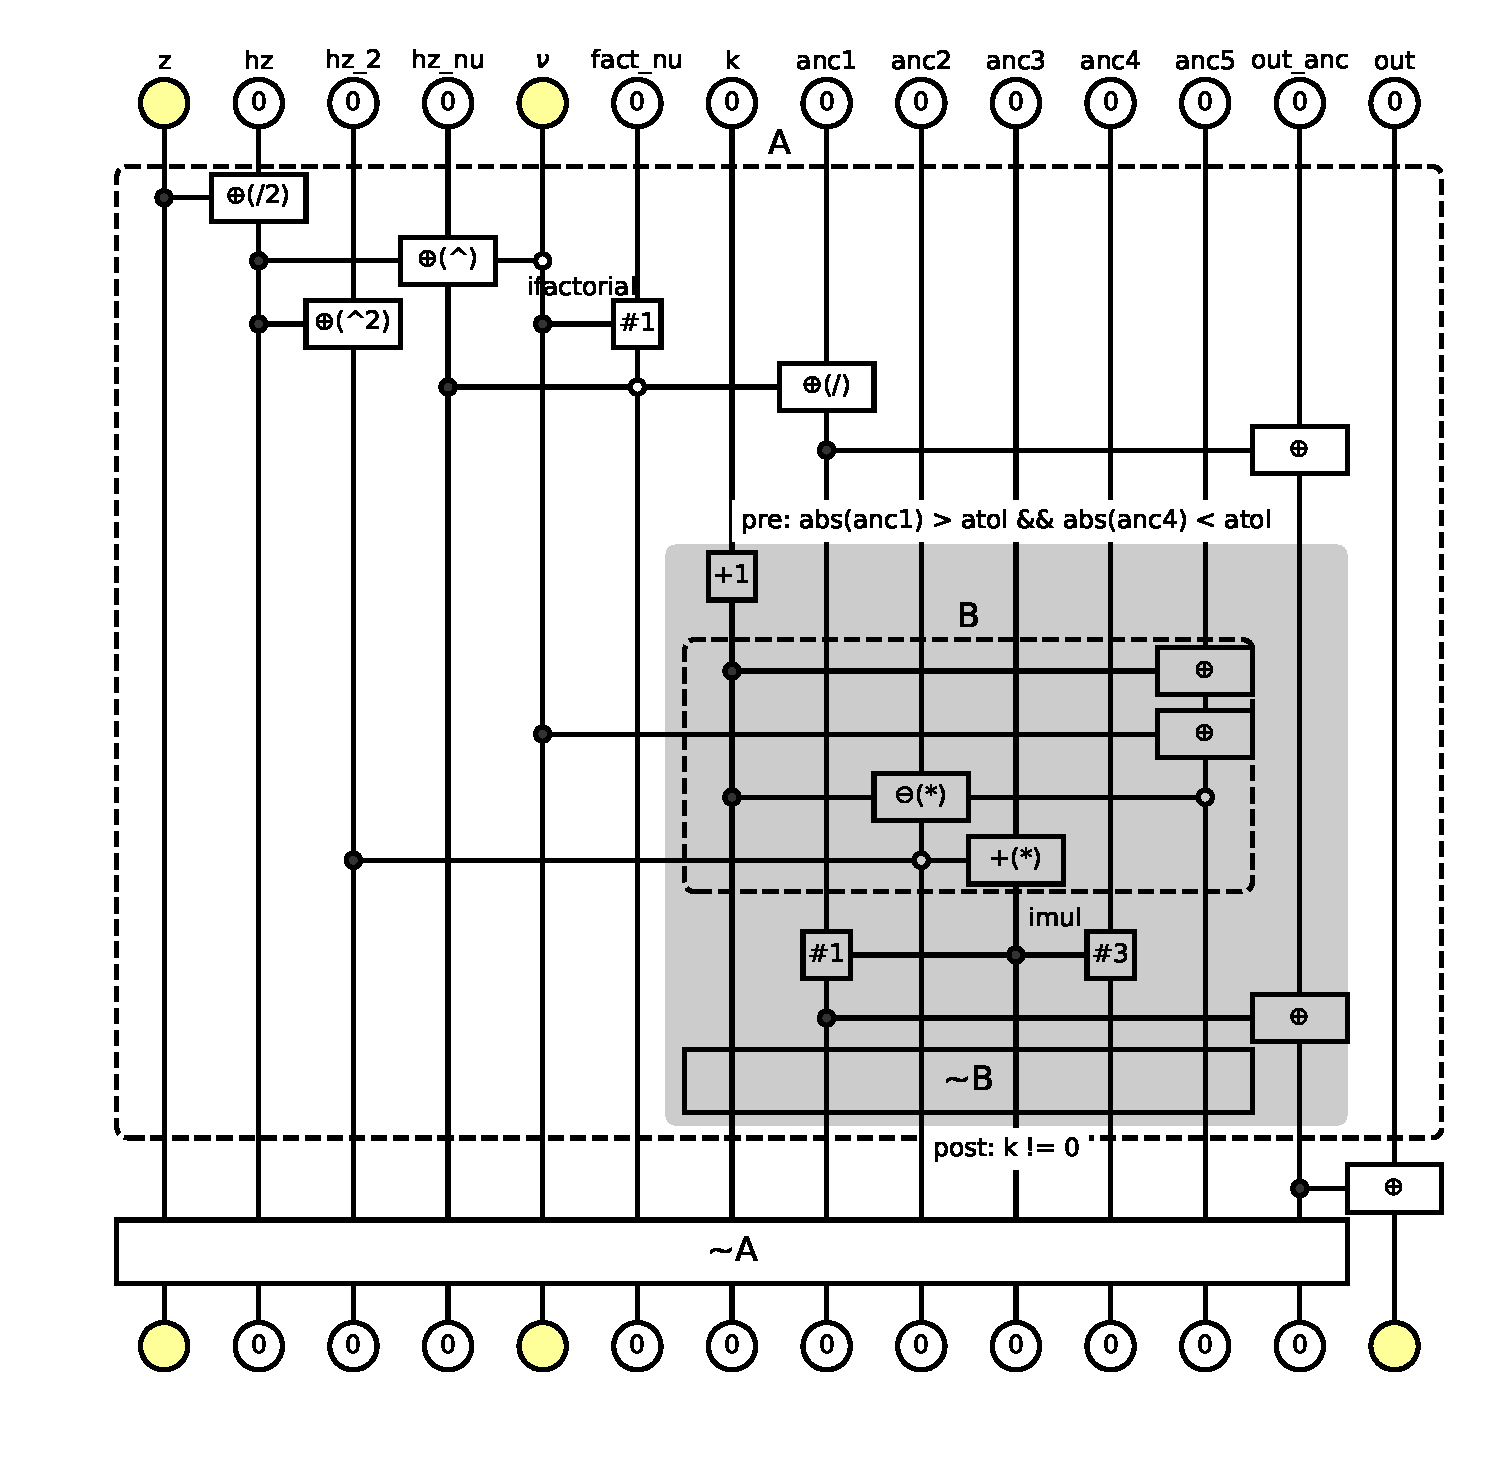
\includegraphics[width=\columnwidth,trim={0 1cm 0 0cm},clip]{images/fig4.pdf}
        \caption{Vertical lines are variables, boxes, and dots connected by parallel lines are operations. A dot represents using a variable as control while a box represents mutating a variable. 
        The gray box represents the body of a while loop. A precondition and postcondition are positioned on its top and bottom.}\label{fig:datagraph}
    \end{subfigure}
    \caption{The comparison between (a) tranditional and (b) memory oriented computational graph of the first kind Bessel function.}\label{fig:cgraphs}
\end{figure*}

In the following, we introduce the reversible implementation and the memory oriented computational graph.
The above Bessel function contains a loop with irreversible ``\texttt{*=}'' operation inside.
Intuitively, consequtive multiplication requires an increasing size of tape to cache the intermediate state $s_n$, since one can not release state $s_{n-1}$ directly after computing $s_n$~\cite{Perumalla2013}.
To reduce the memory allocation without increasing the time complexity of the program, we introduce the following reversible approximate multiplier.

\begin{minipage}{.44\textwidth}
    \begin{lstlisting}[numberstyle=\scriptsize\color{gray},numbers=left,numbersep=8pt]
@i @inline function imul(out!, x, anc!)
    anc! += out! * x
    out! -= anc! / x
    SWAP(out!, anc!)
end
\end{lstlisting}
\end{minipage}

Here, instruction \texttt{SWAP} exchanges values of two variables, $\texttt{anc!} \approx 0$ is a \textit{dirty ancilla}.
Line 2 computes the result and accumulates it to the dirty ancilla, and we get an approximately correct output in \texttt{anc!}.
Line 3 uncompute \texttt{out!} approximately by using the information stored in \texttt{anc!}, leaving a dirty zero state in register \texttt{out!}.
Line 4 swaps the contents in \texttt{out!} and \texttt{anc!}.
Finally, we have an approximately correct output and a dirtier ancilla.
The ``approximate uncomputing'' trick can be extensively used in practice. It mitigated the artificial irreversibility brought by the number system that we have adopted at the cost of output precision.
The reason why this trick works here lies in the fact that from the mathematics perspective the state in $n$th step $\{s_n, z\}$ contains the same amount of information as its previous state  $\{s_{n-1}, z\}$ except some particular points, it is highly possible to find an equation to uncompute the previous state from the current state.
With this approximate multiplier, we implement $J_\nu$ as follows.

\begin{minipage}{.44\textwidth}
\begin{lstlisting}
using NiLang, NiLang.AD

@i function ibesselj(out!, ν, z; atol=1e-8)
    k ← 0
    fact_nu ← zero(ν)
    halfz ← zero(z)
    halfz_power_nu ← zero(z)
    halfz_power_2 ← zero(z)
    out_anc ← zero(z)
    anc1 ← zero(z)
    anc2 ← zero(z)
    anc3 ← zero(z)
    anc4 ← zero(z)
    anc5 ← zero(z)

    @routine begin
        halfz += z / 2
        halfz_power_nu += halfz ^ ν
        halfz_power_2 += halfz ^ 2
        ifactorial(fact_nu, ν)

        anc1 += halfz_power_nu/fact_nu
        out_anc += identity(anc1)
        while (abs(unwrap(anc1)) > atol &&
                abs(unwrap(anc4)) < atol, k!=0)
            k += identity(1)
            @routine begin
                anc5 += identity(k)
                anc5 += identity(ν)
                anc2 -= k * anc5
                anc3 += halfz_power_2 / anc2
            end
            imul(anc1, anc3, anc4)
            out_anc += identity(anc1)
            ~@routine
        end
    end
    out! += identity(out_anc)
    ~@routine
end
\end{lstlisting}
\end{minipage}

Here, the definition of \texttt{ifactorial} could be found in the appendix. Only a finite number of ancillas used, while the time complexity does not increase compared to its irreversible counterpart.
Ancilla \texttt{anc4} plays the role of \textit{dirty ancilla} in multiplication, it is uncomputed rigorously in the uncomputing stage marked by \texttt{$\sim$@routine}.
%The \texttt{while} statement takes two conditions, the precondition and postcondition. Precondition \texttt{val(anc1) > atol} indicates when to break the forward pass and postcondition \texttt{iplus != 0} indicates when to break the backward pass.

This reversible program can be diagrammatically represented as a memory oriented computational graph as show in \Fig{fig:cgraphs} (\subref{fig:datagraph}).
In this graph, a variable is a vertical line, while a function is a parallel line.
The critical difference to the traditional computational graph is that it adopts a variable oriented view.
A variable can be accessed by multiple functions. Hence it represents a hypergraph rather than a simple graph.
If a function uses a variable but does not change the contents in it, we call this variable a control parameter of this function and put a dot at the cross. Otherwise, if the content is changed, we put a square.
This diagram can be used to analyse uncomputable variables. In this example routine ``B'' uses \texttt{hz\_2}, \texttt{$\nu$} and \texttt{k} as control parameters, and changes the contents in \texttt{anc2}, \texttt{anc3} and \texttt{anc5}.
while the following operation \texttt{imul} does not change these variables.
Hence we can apply the inverse routine \texttt{$\sim$B} to safely restore contents in \texttt{anc2}, \texttt{anc3} and \texttt{anc5}, this is what people called compute-copy-uncompute paradigm.
%After computation, values of \texttt{z} and \texttt{$\nu$} are not changed, while a pre-emptied \texttt{out!} is changed to the desired output.
%The whole function can be represented as
%\begin{figure}[htp]
%    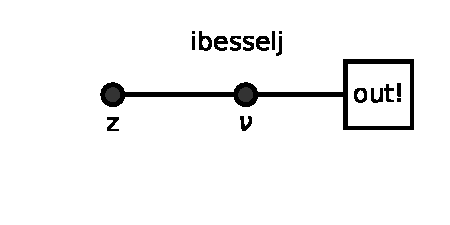
\includegraphics[width=0.4\columnwidth,trim={0cm 1.5cm 0cm 0.5cm},clip]{images/fig5.pdf}
%\end{figure}

%\begin{figure*}
    %\centerline{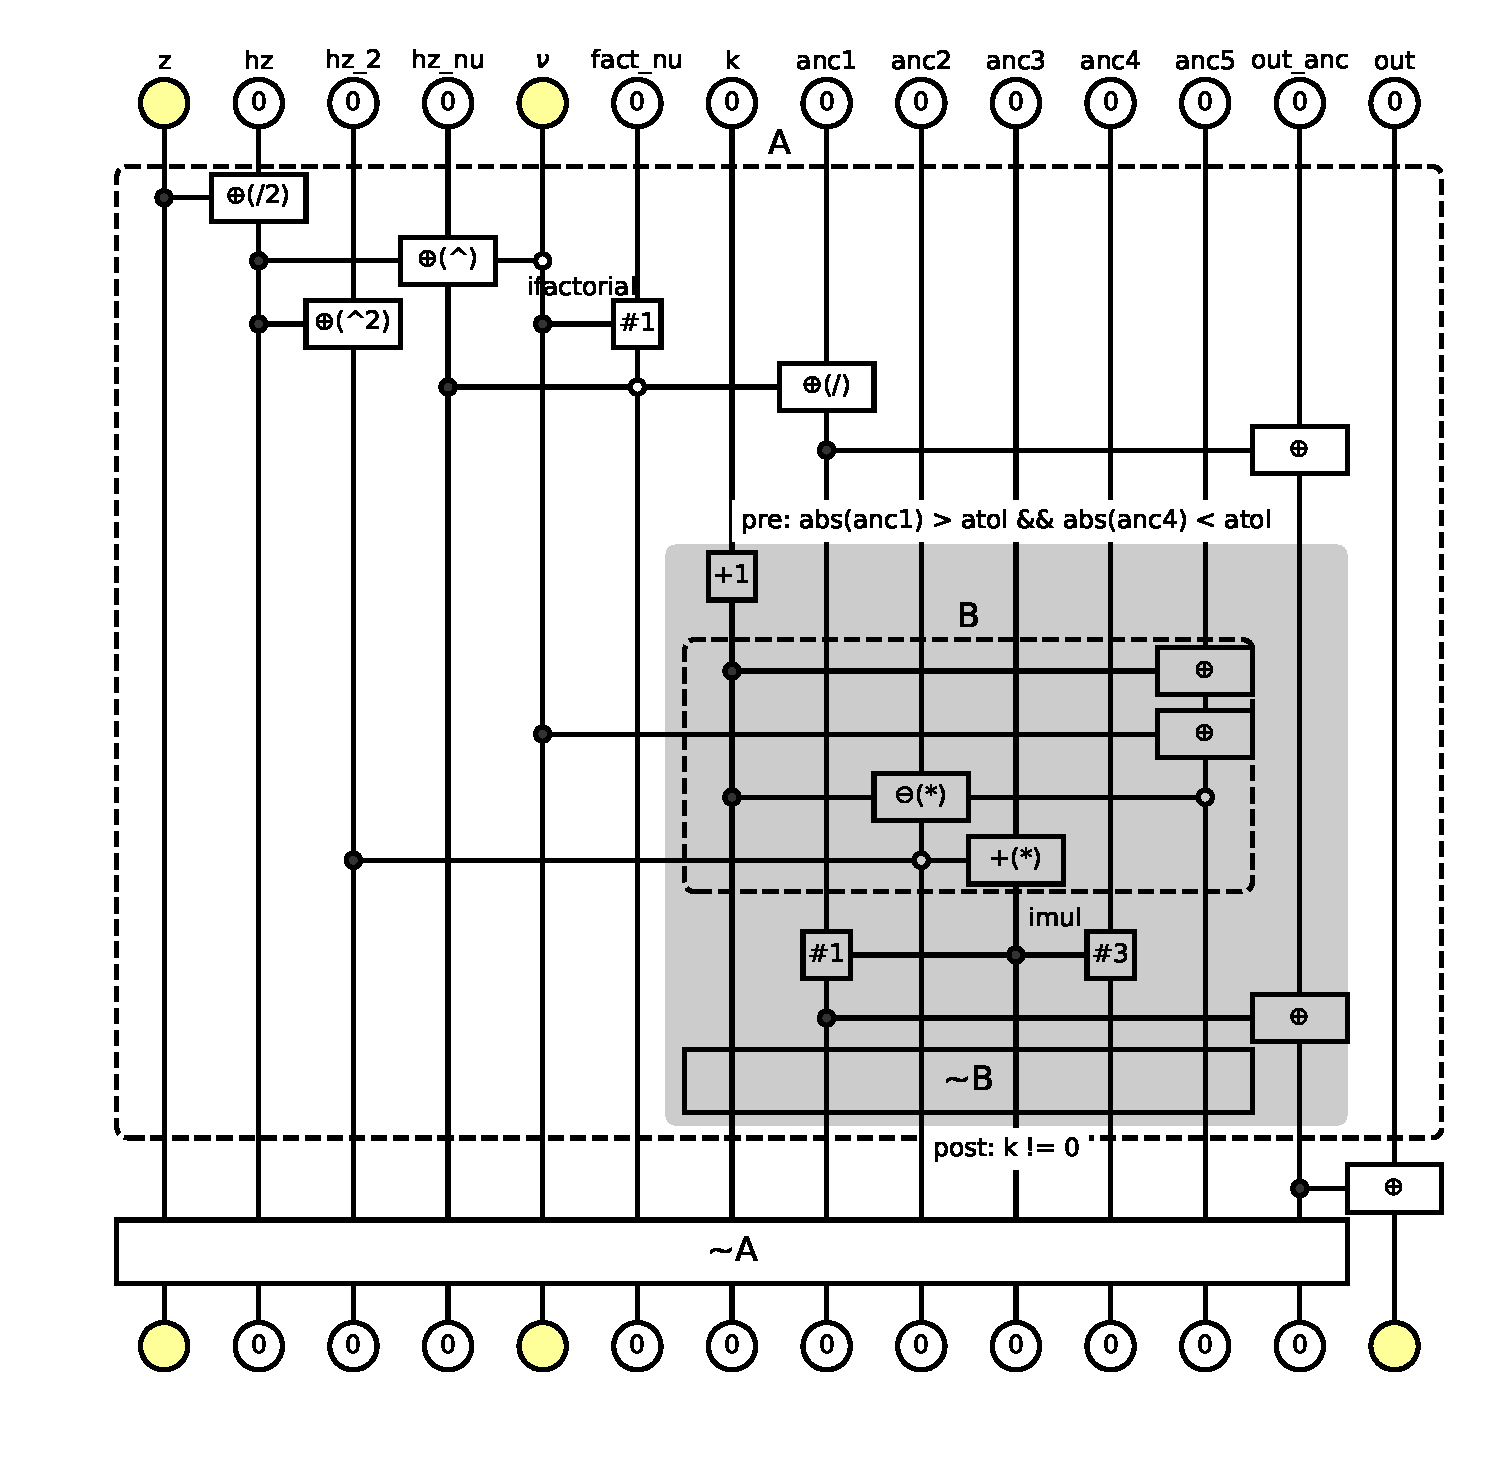
\includegraphics[width=0.7\textwidth,trim={1cm 1cm 0 0},clip]{images/fig4.pdf}}
    %\caption{Data oriented computational graph for the reversible first kind Bessel function. Circles connected by vertical lines are variables, while boxes and dots connected by parallel lines are operations. A dot on a line represents a control parameter while a box represents a mutable parameter. Annotations $\#1, \#2, \ldots$ are used the mark the positions of variables in the argument list. The gray box represents the body of a while loop, where a precondition and postcondition are positioned on top and bottom of this box.}\label{fig:datagraph}
%\end{figure*}

One can obtain gradients of this function by calling \texttt{ibesselj\textquotesingle}.

\begin{minipage}{.44\textwidth}
\begin{lstlisting}
julia> out!, x = 0.0, 1.0
(0.0, 1.0)

julia> ibesselj'(Val(1), out!, 2, x)
(Val{1}(), GVar(0.0, 1.0), 2, GVar(1.0, 0.2102436))
\end{lstlisting}
\end{minipage}

Here, \texttt{ibesselj\textquotesingle} is a callable instance of type \texttt{Grad\{typeof(ibesselj)\}}. The first parameters \texttt{Val(1)} specifies the position of loss in argument list. 
The Hessian can be obtained by feeding dual-numbers into this gradient function.

\begin{minipage}{.44\textwidth}
\begin{lstlisting}
julia> out!, x = 0.0, 1.0
(0.0, 1.0)

julia> ibesselj'(Val(1), out!, 2, x)
(Val{1}(), GVar(0.0, 1.0), 2, GVar(1.0, 0.2102436))

julia> using ForwardDiff: Dual

julia> _, hxout!, _, hxx = ibesselj'(Val(1), 
        Dual(out!, zero(out!)), 2, Dual(x, one(x)));

julia> grad(hxx).partials[1]
0.13446683844358093
\end{lstlisting}
\end{minipage}

Here, the gradient field of \texttt{hxx} is defined as $\frac{\partial {\rm out!}}{\partial x}$, which is a Dual number.
It has a field partials that store the derivative for \texttt{x}.
It corresponds to the Hessian $\frac{\partial{\rm out!}^2}{\partial x^2}$ that we need.
See \App{app:hessian} for alternative approaches to obtain its Hessian.

\subsubsection{Benchmark}
We have different source-to-source automatic differentiation implementations of the first type Bessel function and show the benchmarks below.
\begin{table}[h!]\centering
\begin{minipage}{\columnwidth}
\ra{1.3}
    \scalebox{1.0}{
        \begin{tabularx}{\textwidth}{X X c c}\toprule
            & \textbf{Mode} & \textbf{$T_{\rm min}$/ns} & Space/KB\\
            \hline
            Julia & -- & 22 & 0\\
            NiLang (call/uncall) & -- & 61 & 0\\
            ForwardDiff & Tangent & 35 & 0\\
            Manual & Adjoint & 83 & 0\\
            NiLang.AD & Adjoint & 271 & 0\\
            NiLang.AD (GPU) & Adjoint & 1.4 & 0\\
            Zygote & Adjoint & 31201 & 13.47\\
            %Tapenade & Adjoint & ? & ?\\
            \hline
            \bottomrule
        \end{tabularx}
    }
    \caption{Time and space used in computing the gradients of Bessel function $J_2(1.0)$.
    The CPU device is Intel(R) Xeon(R) CPU E5-2680 v4 @ 2.40GHz, and the GPU device is Nvidia Titan V.
    The GPU time is estimated by broadcasting the gradient function on CUDA array of size $2^{17}$ and take the average.}\label{tbl:besselj}
\end{minipage}
\end{table}

In \Tbl{tbl:besselj}, Julia is the CPU time used for running the irreversible forward program. It is the baseline for benchmarking.
NiLang (call/uncall) is the time of reversible call or uncall. Both of them are 2.8 times slower than its irreversible counterpart. Here, we have removed the reversibility check. Otherwise, it will take more time than this. One can always turn off this check after ruling out possible bugs.
ForwardDiff gives the best performance, and it is even faster than manually derived gradients
\begin{equation}
    J_{\nu}'(z) = \frac{J_{\nu-1} - J_{\nu+1}}{2}.
\end{equation}
Except the efficient implementation, its high performance also lies in the fact that this functions is suited for tangent mode AD which has only one input.
NiLang.AD represents the reversible AD in NiLang, and it takes 12.3 times the original program, which is still is much faster than naive checkpointing.
In Zygote, the memory allocation on the heap is 13.47KB. They are not all for checkpointing. Some of them are related to type instability, where Julia compiler fails to infer types.
Using closure to handle checkpointing can induce poor performance because external type instability sometimes can propagate to the interior.
NiLang uses uncomputing to manage memory rather than closure, which does not frequently involve external variables in the function.
Hence it is more friendly to type inference in Julia compiler.
%Tapenade \blue{needs your effort, @MLS}
We also include a CUDA benchmark. Our reversible programming is compatible with CUDA programming so that the differentiable kernel can be executed on GPU.
For people who are interested in CUDA programming, we prepared another example in \App{app:cuda}, which implements a differentiable quantum simulation kernel on GPU.
So far, the generated backward rule faces the shared write problem, which requires further investigation.

\subsection{Sparse Matrices}
Source to source automatic differentiation is useful in differentiating sparse matrices. It is a well-known problem that sparse matrix operations can not benefit directly from generic backward rules for dense matrix because general rules do not keep the sparse structure.
In the following, we will show that reversible AD can differentiate the Frobenius dot product between two sparse matrices with a state of the art performance. Here, the Frobenius dot product is defined as \texttt{trace(A'B)}.
This following reversible implementation is adapted from the irreversible implementation in Julia package \texttt{SparseArrays}.

\begin{minipage}{.44\textwidth}
\begin{lstlisting}
using SparseArrays

@i function dot(r::T, A::SparseMatrixCSC{T},
        B::SparseMatrixCSC{T}) where {T}
    m ← size(A, 1)
    n ← size(A, 2)
    @invcheckoff branch_keeper ← zeros(Bool, 2*m)
    @safe size(B) == (m,n) || 
        throw(DimensionMismatch(
        "matrices must have the same dimensions"))
    @invcheckoff @inbounds for j = 1:n
        ia1 ← A.colptr[j]
        ib1 ← B.colptr[j]
        ia2 ← A.colptr[j+1]
        ib2 ← B.colptr[j+1]
        ia ← ia1
        ib ← ib1
        @inbounds for i=1:ia2-ia1+ib2-ib1-1
            ra ← A.rowval[ia]
            rb ← B.rowval[ib]
            if (ra == rb, ~)
                r += A.nzval[ia]' * B.nzval[ib]
            end
            # b move -> true, a move -> false
            branch_keeper[i] ⊻= ia == ia2-1 ||
                ra > rb
            ra → A.rowval[ia]
            rb → B.rowval[ib]
            if (branch_keeper[i], ~)
                ib += identity(1)
            else
                ia += identity(1)
            end
        end

        ~@inbounds for i=1:ia2-ia1+ib2-ib1-1
            # b move -> true, a move -> false
            branch_keeper[i] ⊻= ia == ia2-1 ||
                    A.rowval[ia] > B.rowval[ib]
            if (branch_keeper[i], ~)
                ib += identity(1)
            else
                ia += identity(1)
            end
        end
    end
    @invcheckoff branch_keeper → zeros(Bool, 2*m)
end
\end{lstlisting}
\end{minipage}

With simple adaptation, the code becomes reversible.
Here, the key point is using a \texttt{branch\_keeper} vector to cache branch decisions.
In the following example, we compare the time used in the forward pass and backward pass.

\begin{minipage}{.44\textwidth}
\begin{lstlisting}
julia> using BenchmarkTools

julia> a = sprand(1000, 1000, 0.01);

julia> b = sprand(1000, 1000, 0.01);

julia> @benchmark SparseArrays.dot($a, $b)
BenchmarkTools.Trial: 
  memory estimate:  0 bytes
  allocs estimate:  0
  --------------
  minimum time:     94.537 μs (0.00% GC)
  median time:      96.959 μs (0.00% GC)
  mean time:        98.188 μs (0.00% GC)
  maximum time:     189.291 μs (0.00% GC)
  --------------
  samples:          10000
  evals/sample:     1

julia> out! = SparseArrays.dot(a, b)
25.19659286755114

julia> @benchmark (~dot)($(GVar(out!, 1.0)),
        $(GVar.(a)), $(GVar.(b)))
BenchmarkTools.Trial:   #$ TODO: remove this comment
  memory estimate:  2.17 KiB
  allocs estimate:  2
  --------------
  minimum time:     151.392 μs (0.00% GC)
  median time:      153.153 μs (0.00% GC)
  mean time:        155.884 μs (0.00% GC)
  maximum time:     270.534 μs (0.00% GC)
  --------------
  samples:          10000
  evals/sample:     1
\end{lstlisting}
\end{minipage}

The time used for computing backward pass costs is approximately 1.6 times Julia's native forward pass.
Here, we have turned off the reversibility check off to achieve better performance.
By writing sparse matrix multiplication and other sparse matrix operations reversibly,
we will have a differentiable sparse matrix library with proper performance.

\subsection{Unitary Matrices}\label{sec:umm}
A unitary matrix features uniform eigenvalues and reversibility. It is widely used as an approach to ease the gradient exploding and vanishing problem~\cite{Arjovsky2015,Wisdom2016,Li2016} and the memory wall problem~\cite{Luo2019}.
One of the simplest ways to parametrize a unitary matrix is representing a unitary matrix as a product of two-level unitary operations~\cite{Li2016}. A real unitary matrix of size $N$ can be parametrized compactly by $N(N-1)/2$ rotation operations~\cite{Li2013}
\begin{align}
    {\rm ROT}(a!, b!, \theta)  = \left(\begin{matrix}
        \cos(\theta) & - \sin(\theta)\\
        \sin(\theta)  & \cos(\theta)
    \end{matrix}\right)
    \left(\begin{matrix}
        a!\\
        b!
    \end{matrix}\right),
\end{align}
where \texttt{$\theta$} is the rotation angle, \texttt{a!} and \texttt{b!} are target registers.

\begin{minipage}{.44\textwidth}
\begin{lstlisting}[mathescape=true]
using NiLang, NiLang.AD

@i function umm!(x!, θ)
    @safe @assert length(θ) == 
            length(x!)*(length(x!)-1)/2
    k ← 0
    for j=1:length(x!)
        for i=length(x!)-1:-1:j
            k += identity(1)
            ROT(x![i], x![i+1], θ[k])
        end
    end

    k → length(θ)
end
\end{lstlisting}
\end{minipage}

Here, the ancilla \texttt{k} is deallocated manually by specifying its value, because we know the loop size is $N(N-1)/2$.
We define the test functions in order to check gradients.

\begin{minipage}{.44\textwidth}
\begin{lstlisting}[mathescape=true]
julia> @i function test!(out!, x!::Vector, θ::Vector)
           umm!(x!, θ)
           isum(out!, x!)
       end

julia> out, x, θ = 0.0, randn(4), randn(6);

julia> @instr test!'(Val(1), out, x, θ)

julia> x
4-element Array{GVar{Float64,Float64},1}:
 GVar(1.220182125326287, 0.14540743042341095) 
 GVar(2.1288634811475937, -1.3749962375499805)
 GVar(1.2696579252569677, 1.42868739498625)   
 GVar(0.1083891125379283, 0.2170123344615735) 

julia> @instr (~test!')(Val(1), out, x, θ)

julia> x
4-element Array{Float64,1}:
 1.220182125326287  
 2.1288634811475933 
 1.2696579252569677 
 0.10838911253792821
\end{lstlisting}
\end{minipage}

In the above testing code, \texttt{test\textquotesingle} attaches a gradient field to each element of \texttt{x}. \texttt{$\sim$test\textquotesingle} is the inverse program that erase the gradient fields.
Notably, this reversible implementation costs zero memory allocation, although it changes the target variables inplace.

%It implements the backward rule of a \texttt{ROT} instruction
%\begin{align}
%    \begin{split}
%    \overline{\theta}  &= \sum\frac{\partial R(\theta)}{\partial \theta}\odot(\overline{out!}x^T)\\
%    &= \Tr\left[\frac{\partial R(\theta)}{\partial \theta}^T\overline{out!}x^T\right]\\
%    &= \Tr\left[R\left(\frac{\pi}{2}-\theta\right)\overline{out!}x^T\right]
%    \end{split}
%\end{align}

\subsection{QR decomposition}

Let us consider a naive implementation of QR decomposition from scratch.
We admit this implementation is just a proof of principle which does not consider reorthogonalization and other practical issues.

\begin{minipage}{.44\textwidth}
\begin{lstlisting}
using NiLang, NiLang.AD

@i function qr(Q, R, A::Matrix{T}) where T
    anc_norm ← zero(T)
    anc_dot ← zeros(T, size(A,2))
    ri ← zeros(T, size(A,1))
    for col = 1:size(A, 1)
        ri .+= identity.(A[:,col])
        for precol = 1:col-1
            dot(anc_dot[precol], Q[:,precol], ri)
            R[precol,col] += 
                identity(anc_dot[precol])
            for row = 1:size(Q,1)
                ri[row] -= 
                    anc_dot[precol] * Q[row, precol]
            end
        end
        norm2(anc_norm, ri)

        R[col, col] += anc_norm^0.5
        for row = 1:size(Q,1)
            Q[row,col] += ri[row] / R[col, col]
        end

        ~begin
            ri .+= identity.(A[:,col])
            for precol = 1:col-1
                dot(anc_dot[precol], Q[:,precol], ri)
                for row = 1:size(Q,1)
                    ri[row] -= anc_dot[precol] *
                        Q[row, precol]
                end
            end
            norm2(anc_norm, ri)
        end
    end
end
\end{lstlisting}
\end{minipage}

Here, in order to avoid frequent uncomputing, we allocate ancillas \texttt{ri} and \texttt{anc\_dot} as vectors.
The expression in $\sim$ is used to uncompute \texttt{ri}, \texttt{anc\_dot} and \texttt{anc\_norm}.
\texttt{dot} and \texttt{norm2} are reversible functions to compute dot product and vector norm.
One can easily quickly the correctness of the gradient function

\begin{minipage}{.44\textwidth}
\begin{lstlisting}
julia> A  = randn(4,4);

julia> q, r = zero(A), zero(A);

julia> @i function test1(out, q, r, A)
           qr(q, r, A)
           isum(out, q)
       end

julia> check_grad(test1, (0.0, q, r, A); iloss=1)
true
\end{lstlisting}
\end{minipage}

Here, the loss function \texttt{test1} is defined as the sum of the output unitary matrix \texttt{q}. The \texttt{check\_grad} function is a gradient checker function defined in module NiLang.AD.

\subsection{Solving a graph embedding problem}\label{sec:graph}
Graph embedding can be used to find representation for an order parameter~\cite{Takahashi2020} in condensed matter physics.
\Ref{Takahashi2020} considers a problem of finding the minimum Euclidean space dimension $k$ that a Petersen graph can fit into, with extra requirements that the distance between a pair of connected vertices has the same value $l_1$, the distance between a pair of disconnected vertices has the same value $l_2$ and $l_2 > l_1$.
The Petersen graph is ten vertices graph, as shown in \Fig{fig:petersen}.\begin{figure}
    \centerline{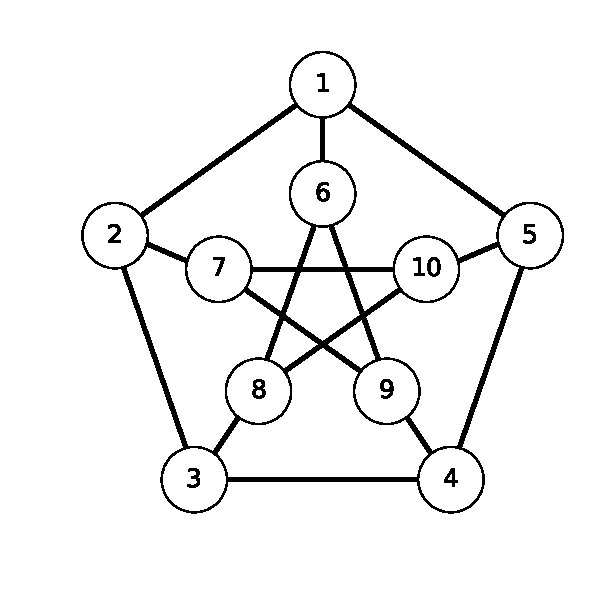
\includegraphics[width=0.6\columnwidth,trim={0 1cm 0 0},clip]{images/petersen.pdf}}
    \caption{The Petersen graph with 10 vertices and 15 edges.}\label{fig:petersen}
\end{figure}
Let us denote the set of connected and disconnected vertex pairs as $L_1$ and $L_2$, respectively. This problem can be variationally solved by differential programming by designing the subsequent loss.
\begin{align}
    \begin{split}
        \mathcal{L} &= \Var({\rm dist}(L_1)) + \Var({\rm dist}(L_2)) \\
        &+\exp({\rm relu}(\overline{{\rm dist}(L_1)} - \overline{{\rm dist}(L_2)} + 0.1))) - 1
    \end{split}
\end{align}
The first line is a summation of distance variances in two sets of vertex pairs, where $\Var{X}$ means taking the variance of samples in $X$.
The second line is used to guarantee $l_2 > l_1$, where $\overline{X}$ means taking the average of samples in $X$.
Its reversible implementation is shown below.

\begin{minipage}{.44\textwidth}
\begin{lstlisting}
using NiLang, NiLang.AD

@i function sqdistance(dist!, x1::AbstractVector{T},
        x2::AbstractVector) where T
    @inbounds for i=1:length(x1)
        x1[i] -= identity(x2[i])
        dist! += x1[i] ^ 2
        x1[i] += identity(x2[i])
    end
end

# bonds of a petersen graph
const L1 = [(1, 6), (2, 7), (3, 8), (4, 9), (5, 10),
    (1, 2), (2, 3), (3, 4), (4, 5), (1, 5), (6, 8),
    (8, 10), (7, 10), (7, 9), (6, 9)]

# disconnected bonds of a petersen graph
const L2 = [(1, 3), (1, 4), (1, 7), (1, 8), (1, 9),
    (1, 10), (2, 4), (2, 5), (2, 6), (2, 8), (2, 9),
    (2, 10), (3, 5), (3, 6), (3, 7), (3, 9), (3, 10),
    (4, 6), (4, 7), (4, 8), (4, 10), (5, 6), (5, 7),
    (5, 8), (5, 9), (6, 7), (6, 10), (7, 8), (8, 9),
    (9, 10)]

@i function embedding_loss(out!::T, x) where T
    v1 ← zero(T)
    m1 ← zero(T)
    v2 ← zero(T)
    m2 ← zero(T)
    diff ← zero(T)
    d1 ← zeros(T, length(L1))
    d2 ← zeros(T, length(L2))
    @routine begin
        for i=1:length(L1)
            sqdistance(d1[i], 
                x[:,L1[i][1]],x[:,L1[i][2]])
        end
        for i=1:length(L2)
            sqdistance(d2[i],
                x[:,L2[i][1]],x[:,L2[i][2]])
        end
        var_and_mean_sq(v1, m1, d1)
        var_and_mean_sq(v2, m2, d2)
        m1 -= identity(m2)
        m1 += identity(0.1)
    end
    out! += identity(v1)
    out! += identity(v2)
    if (m1 > 0, ~)
        # to ensure mean(v2) > mean(v1)
        # if mean(v1)+0.1 - mean(v2) > 0, punish it.
        out! += exp(m1)
        out! -= identity(1)
    end
    ~@routine
end
\end{lstlisting}
\end{minipage}

One can access the gradient by typing

\begin{minipage}{.44\textwidth}
\begin{lstlisting}
julia> embedding_loss'(Val(1), 0.0, randn(5, 10))
\end{lstlisting}
\end{minipage}

One can also obtain the Hessian with the following function

\begin{minipage}{.44\textwidth}
\begin{lstlisting}
using ForwardDiff: Dual, partials

function get_hessian(params0::AbstractArray{T}) where T
    N = length(params0)
    params = Dual.(params0, zero(T))
    hes = zeros(T, N, N)
    @inbounds for i=1:N
        i !== 1 && (params[i-1] =
            Dual(params0[i-1], zero(T)))
        params[i] = Dual(params0[i], one(T))
        res = gradient(Val(1), embedding_loss,
            (Dual(0.0, 0.0), params))[2]
        hes[:,i] .= vec(partials.(res, 1))
    end
    hes
end
\end{lstlisting}
\end{minipage}

We repeat the training for each dimension $k$ from $1$ to $10$ and search for possible solutions by variationally optimizing the positions of vertices.
In each training, we fix two of the vertices and train the rest. Otherwise, the program will find the trivial solution with overlapped vertices. 
For $k=5$, we can get a loss close to machine precision with high probability, while for $k < 5$, the loss is always much higher than $0$.
From the solution, it is easy to see $l_2/l_1 = \sqrt{2}$ is the solution.
For $k=5$, an Adam optimizer with a learning rate $0.01$~\cite{Kingma2014} requires $\sim2000$ steps training.
The trust region Newton's method converges much faster, which requires $\sim 20$ computations of Hessians to reach convergence.
Although training time is comparable, the converged precision of the later is much better.

\subsubsection{Benchmark}
Since the ForwardDiff itself provides the Hessian for users. It is interesting to benchmark how much performance we can get by forward differentiating an adjoint program than forward differentiating a forward AD program.
\begin{figure}
    \centerline{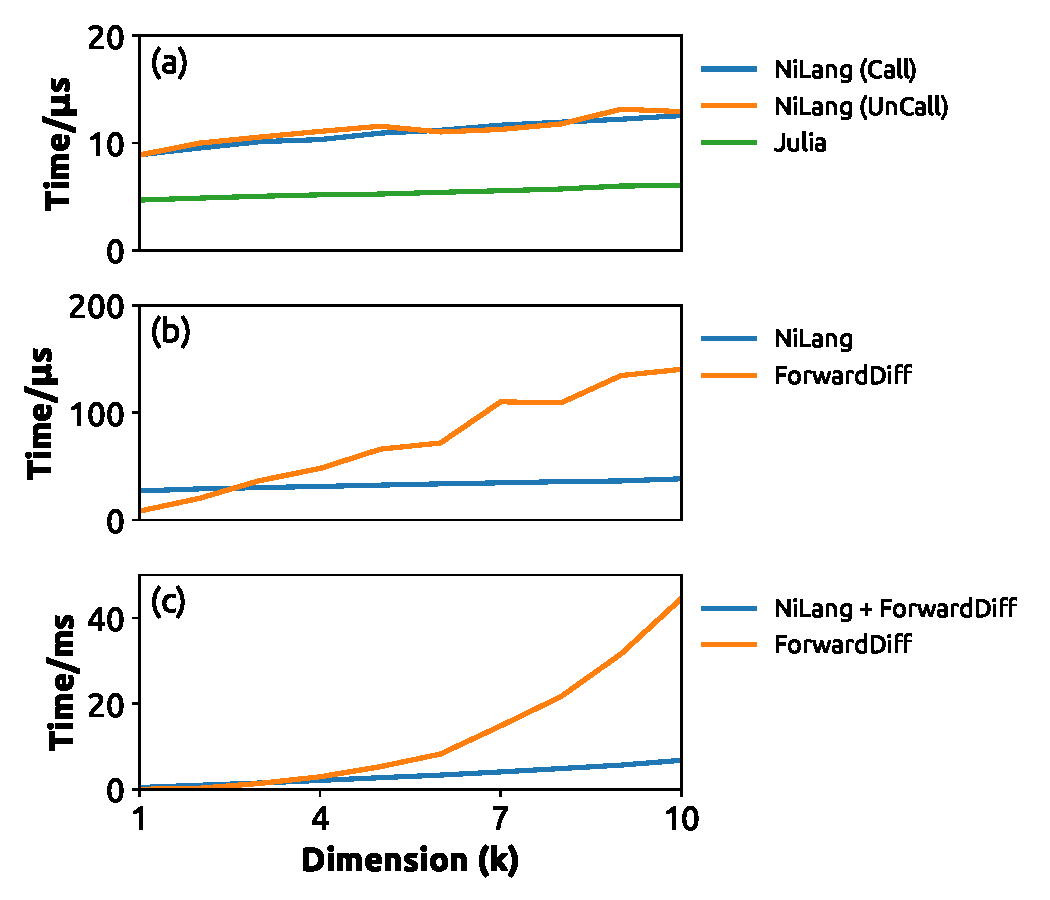
\includegraphics[width=\columnwidth,trim={0 0 0 0},clip]{images/fig7.pdf}}
    \caption{The time used to (a) call/uncall, (b) compute gradients and (c) compute Hessians.}\label{fig:bench-embedding}
\end{figure}
The benchmark is on GPU, which uses the same setup as previous benchmarks.
In this application, the number of input parameters scales as $10 \times k$, where $k$ is the embedding dimension of the graph.
In \Fig{fig:bench-embedding}, we show the the performance of different implementations by varying the dimension $k$.
As the baseline, (a) shows the time for computing the 0th-order gradient, or the function call. We have reversible and irreversible implementations, where the reversible program is slower than the irreversible native Julia program by a factor of $\sim2$.
(b) shows the time for computing the first-order gradients. The reversible program shows the advantage of obtaining gradients when the dimension $k \geq 3$. The larger the number of inputs, the more advantage it shows due to the overhead proportional to input size in tangent mode AD.
The same reason applies to compute Hessians. The mixed-mode AD gives better performance when $k \geq 3$ comparing with pure tangent mode AD.

\section{Discussion and outlook}\label{sec:discussion}
In this paper, we show how to realize a reversible programming eDSL and how to implement source-to-source adjoint mode AD on top of it.
It gives the user more flexibility to tradeoff memory and computing time comparing with traditional checkpointing.
The Julia implementation NiLang gives a state of the art performance and memory efficiency in obtaining first and second-order gradients in applications including first type Bessel function, sparse matrix manipulation, linear algebra functions and a practical, the application graph embedding problem.
%In a reversible programming language, we proposed to use ``approximate uncomputing'' trick to avoid the overhead of a reversible program in many practical cases.

In the following, we discussed some practical issues about reversible programming, and several future directions to go.
%Notablely, we introduce the concept of ``arithematic uncomputing'' to reduce the overhead of recursive reversible algorithms.

\subsection{Time Space Tradeoff}\label{sec:timespace}
In history, there have been many discussions about time-space tradeoff on a reversible Turing machine (RTM).
In the most straightforward g-segment tradeoff scheme~\cite{Bennett1989,Levine1990}, an RTM model has either a space overhead that is proportional to computing time $T$ or a computational overhead that sometimes can be exponential to the program size comparing with an irreversible counterpart.
This result stops many people from taking reversible computing seriously as a high-performance computing scheme.
In the following, we try to convince the readers that the overhead of reversible computing is not as terrible as people thought.
%we have
%\begin{align}
%    Time(T) &= \frac{T^{1+\epsilon}}{S^\epsilon},\\
%    Space(T) &= \epsilon 2^{1/\epsilon}(S+S\log\frac{T}{S}).
%\end{align}
%Here, $T$ and $S$ are the time and space usage on a irreversible Turing machine. $\epsilon$ is the control parameter.
%It is related to the g-segment trade off parameters by $g = k^n, \epsilon = \log_k(2k-1)$ with $n\geq 1$ and $k\geq 1$.
%First, let $\epsilon \rightarrow 0$, there is not overhead in time. 

The overhead of reversing a program is bounded the checkpointing~\cite{Chen2016} strategy used in a traditional machine learning package that memorizes inputs of primitives because similar strategy can also be used in reversible programming.~\cite{Perumalla2013}
% Memorizing the inputs always make a primitive reversible since it does not discard any information.
%For deep neural networks, people used checkpointing trick to trade time with space~\cite{Chen2016}. This trick is also widely used in reversible programming~\cite{Perumalla2013}. 
Reversible programming provides more alternatives to reduce the overhead.
%For inplace functions, especially those reversible functions. Reversible programming AD is sometimes more memory efficient. Comparing with logging computational graph.
%Second, many computational overheads come from of the irreversibility of \texttt{/=} and \texttt{*=} operations. This part is not fundamental because reversible floating point instructions have already been designed~\cite{Nachtigal2010,Nachtigal2011}. Using reversible floating point instructions may significant decrease the computation time and memory usage of a RTM.
%Even in current stage, 
For example, accumulation is reversible, and it does not require checkpointing.
The checkpointing in many iterative algorithms can often be avoided with the ``arithmetic uncomputing'' trick without sacrificing reversibility, as shown in the \texttt{ibesselj} example in \Sec{sec:bessel}.
% We will review this point in \Sec{sec:hardware}.

As shown in \Fig{fig:ccu}, clever compiling based on memory oriented computational graph can also be used to help user tradeoff between time and space.
Often, when we define a new reversible function, we allocate some ancillas at the beginning of the function and deallocate them through uncomputing at the end.
The overhead comes from the uncomputing. In the worst case, the time used for uncomputing can be the same as the forward pass.
In a hierarchical design, uncomputing can appear in every layer of abstraction. To quantify the overhead of uncomputing, we introducing the term program granularity as bellow.
\begin{definition}[program granularity]
    The log-ratio between the execution time of a reversible program and its irreversible counterpart.
\end{definition}
The computing time increases exponentially as the granularity increases.
A cleverer compilation of a program can reduce the granularity by merging the uncomputing statements to avoid repeated efforts.

At last, making reversible programming an eDSL rather than an independent language allows flexible choices between reversibility and computational overhead. For example, to deallocate the memory that stores gradients in a reversible language, one has to uncompute the whole process of obtaining them.
As an eDSL, one has an alternative to deallocate the memory irreversibly outside the scope of a reversible program, i.e., trade energy with time.


%One should notice the memory advantage of reversible programming to machine learning does comes from reversibility itself, but from a better data tracking strategy inspired from invertible programming.
%Normally, a reversible program is not as memory efficient as its irreversible couterpart due to the additional requirement of no information loss. A naive approach that keeping track of all information will cost an additional space $O(T)$, where $T$ stands for the excution time in a irreversible TM, the longer the program runs, the larger the memory usage is. This is exactly the approach to keeping reversibility in most machine learning packages in the market.
%The point it, an reversible Turing Machine is able to trade space with time.
%In some cases, it may cause polynomial overhead than its irreversible counterpart.

\subsection{Instructions and Hardwares}\label{sec:hardware}
%Todays CPU are starving, that is, the memory access is the performance bottleneck in many applications rather than the arithmetic operations.
%There is a natural granularity for operations with memory access or not.
So far, our eDSL is compiled to Julia.
In the future, it can be compiled to reversible instructions~\cite{Vieri1999} and executed on a reversible device.
%For example, the control flow defined in this NiLang can be compiled to reversible instructions like reversible \texttt{goto} instruction, where
%the target instruction can be a \texttt{comefrom} instruction that specifing the postcondition.
However, arithmetic instructions should be redesigned to support better reversible programs.
The major obstacle to exact reversibility programming is the current floating-point adders and multipliers used in our computing devices are not exactly reversible.
There are proposals of reversible floating -oint adders and multipliers~\cite{Nachtigal2010,Nachtigal2011,Nguyen2013,Hner2018}. However these designs require allocating garbage bits in each operation.
%, which is not too different from the information buffer approach~\cite{Maclaurin2015}.
%In other words, to represent a 64 bit floating point number requires more than 64 bits in storage. Reversible multiplier is also possible in similar approach.~\cite{Nachtigal2010} 
%With floating point numbers, rigorous reversible arithematic designs without using information buffer or garbage qubits is nearly impossible.
Alternatives include fixed point numbers~\cite{FixedPointNumbers} and logarithmic numbers~\cite{Taylor1988,LogarithmicNumbers}, where logarithmic number system is reversible under \texttt{*=} and \texttt{/=}.
We also need instructions like \texttt{comefrom} as a partener of \texttt{goto}.
Many people know \texttt{comefrom} from the joke~\cite{COMEFROM}~\footnote{I heard this joke from Damian Steiger when we were discussing his quantum simulation paper~\cite{Haner2017}.} to complaint people who use \texttt{goto} frequently.
It turns out to be necessary for compiling a reversible program.

%Reversible programming is not nessesarily related to reversible hardwares.
%Reversible programs is a subset of irreversible programs, hence can be simulated efficiently on traditional CMOS devices~\cite{Vieri1999}.
%Reversible programming just provides an alternative to execute on an energy efficient reversible hardwares.
Reversible instructions can be executed on energy-efficient reversible hardware.
In the introduction, we mentioned several reversible hardware. Reversible hardware can be devices supporting reversible gates like the Toffoli gate and the Fredkin gate, or devices like an adiabatic CMOS with the ability to recover signal energy. The latter is known as the generalized reversible computing.~\cite{Frank2005,Frank2017b}
It is already a better choice as the computing device in a spacecraft~\cite{Debenedictis2017}.
Since reversible programming is an exceptional platform for differential programming, building an energy-efficient artificial intelligence (AI) coprocessors would be a promising direction to go too.
%Since reversible computing is mainly driven by quantum computing in recent years.
%In the following, we comment briefly on quantum devices.

The development of reversible compiling theory can be benefit quantum compiling directly.
It bridges classical computing and quantum computing.
Building a universal quantum computer~\cite{Nielsen2002} is difficult. 
The difficulty lies in the fact that it is hard to protect a quantum state.
Unlike a classical state, a quantum state can not be cloned. Meanwhile, it loses information by interacting with the environment.
%These two facts underlines the simulation nature of quantum devices.
%Although there are proposals about quantum random access memory~\cite{Giovannetti2008}, they are difficult to implement, and are known to have many caveats~\cite{Aaronson2015}.
%In the era of noisy intermediate sized quantum devices, more and more people are switching to classical-quantum hybrid devices, where a quantum device plays the role of a programmable simulator.
Classical reversible computing does not enjoy the quantum advantage, nor the quantum disadvantages of non-cloning and decoherence.
%The reversibility of quantum computing comes from the fact that microscopic processes are unitary.
%On the other side, the irreversibility is rare, it can come from interacting with classical devices. Irreversible processes include decaying, qubit state resetting, measurements and classical feed backs to quantum devices. These are typically harder to implement on a quantum device.
%Given the fundamental limitations of quantum decoherence and non-cloning and the reversible nature of microscopic world.
It is technically more smooth to have a reversible computing device to bridge the gap between classical devices and universal quantum computing devices.
By introducing entanglement little by little, we can accelerate some elementary components in reversible computing. For example, quantum Fourier transformation provides an alternative to the reversible adders and multipliers by introducing the CPHASE quantum gate.~\cite{RuizPerez2017}
Currently, most quantum programming language preassumes a classical coprocessor and use classical control flows~\cite{Svore2018} in universal quantum computing.
However, we believe reversible compiling technologies, including reversible control flows, are also very important to a universal quantum computer.

\subsection{Outlook}\label{sec:outlook}

We can use NiLang to solve many existing issues related to AD.
We can use it to generate AD rules for existing machine learning packages like Zygote~\cite{Innes2019}, KNet~\cite{KNet}, and Flux~\cite{Innes2018a}.
Many backward rules for sparse arrays and linear algebra operations have not been defined yet in these packages.
We can also use the flexible time-space tradeoff in reversible programming to overcome the memory wall problem in some applications.
A successful, related example is the memory-efficient domain-specific AD engine in quantum simulator Yao~\cite{Luo2019}.
This domain-specific AD engine is written in a reversible style and solved the memory bottleneck in variational quantum simulations. It also gives so far the best performance in differentiating quantum circuit parameters.
Similarly, we can write memory-efficient normalizing flow~\cite{Kobyzev2019} with NiLang. Normalizing flow is a successful class of generative models in both computer vision~\cite{Kingma2018} and quantum physics~\cite{Dinh2016,Li2018}, where its building block bijector is reversible.
We can use a similar idea to differentiate reversible integrators~\cite{Hut1995, Laikov2018}.
With reversible integrators, it should be possible to rewrite the control system in robotics~\cite{Giftthaler2017} in a reversible style, where scalar is a first-class citizen rather than tensor.
Writing a reversible control program should boost training performance.
Reversibility is also a valuable resource for training.
We show the potential of self-consistent training in \App{sec:train}.

To solve the above problems better, people can improve reversible programming from multiple perspectives.
First, we need a better compiler suited for compiling reversible programs. It can decrease the uncomputing overheads automatically for us.
A better compiler can also help to avoid the problem of shared memory write problem on GPU when computing gradients.
Then, we need a number system to avoid rounding errors. Currently, we can simulate rigorous reversible arithmetics with the fixed-point number package~\cite{FixedPointNumbers,LogarithmicNumbers}. A more efficient fixed point or log number operations requires instruction-level design.
Finally, the improvement from the hardware level will arm reversible differential programming with energy efficiency, which is also very important to help variational programming to solve practical issues better. For example, we can build an energy-efficient AI chip in our cellular phone with reversible computing devices.
%There are also some known issues to be solved like the type inference problem, we have listed some of them on GitHub.
%NiLang also need better type inference support. Current type inference assumes the variable types not changed by a function, which is not true.
%The type cast rule of a reversible function should be recorded somewhere to help type inference.
These improvements need the participation of people from multiple fields.

% By porting a quantum simulator. 
%it is interesting to see how quantum simulator can improve the instruction design. Notice a quantum fourier transformation (QFT) based quantum adder and multiplier is sometimes more efficient than a classical adder~\cite{Haener2018} \blue{Is this true?}.
%This could be used to reduce the momory cost in normalizing flow, time-reversible integrator, recurrent neural network and residual neural network.

\section{acknowledgments}
Jin-Guo Liu thank Lei Wang for motivating the project with possible applications to reversible integrator, normalizing flow, and neural ODE.
Marisa Kiresame and Xiu-Zhe Luo for discussion on the implementation details of source-to-source automatic differentiation,
Shuo-Hui Li for helpful discussion on differential geometry, Tong Liu and An-Qi Chen for helpful discussion on quantum adders and multipliers, Yin-Bo Ma for correcting typos by submitting pull requests, Chris Rackauckas for helpful discussion on reversible integrator, Mike Innes for reviewing the comments about Zygote, Jun Takahashi for discussion about the graph embedding problem, Simon Byrne and Chen Zhao for helpful discussion on floating-point and logarithmic numbers.
The authors are supported by the National Natural Science Foundation of China under Grant No.~11774398, the Strategic Priority Research Program of Chinese Academy of Sciences Grant No.~XDB28000000.

\bibliographystyle{apsrev4-1}
\bibliography{invc}

\pagebreak
\appendix

\section{NiLang Grammar}\label{app:grammar}

To define a reversible function one can use ``@i'' plus a standard function definition like bellow

\begin{minipage}{.44\textwidth}
\begin{lstlisting}[basicstyle=\small\ttfamily,columns=fullflexible]
"""
docstring...
"""
@i function f(args..., kwargs...) where {...}
    <stmts>
end
\end{lstlisting}
\end{minipage}
where the definition of ``<stmts>'' are shown in the grammar page bellow.
The following is a list of terminologies used in the definition of grammar
\begin{itemize}
    \item $ident$, symbols
    \item $num$, numbers
    \item $\epsilon$, empty statement
    \item $JuliaExpr$, native Julia expression
    \item $[$ $]$,  zero or one repetitions.
\end{itemize}
Here, all $JuliaExpr$ should be pure. Otherwise, the reversibility is not guaranteed.
Dataview is a view of data. It can be a bijective mapping of an object, an item of an array, or a field of an object.

\newpage

\begin{minipage}{0.3\textwidth}
    \small
\begin{bnf*}
    \bnfprod{Stmts}{\bnfsp \bnfes}\\
    \bnfmore{\bnfor \bnfpn{Stmt}}\\
    \bnfmore{\bnfor \bnfpn{Stmts} \bnfsp \bnfpn{Stmt}}\\
    \bnfprod{Stmt}{\bnfpn{BlockStmt}}\\
    \bnfmore{\bnfor \bnfpn{IfStmt}}\\
    \bnfmore{\bnfor \bnfpn{WhileStmt}}\\
    \bnfmore{\bnfor \bnfpn{ForStmt}}\\
    \bnfmore{\bnfor \bnfpn{InstrStmt}}\\
    \bnfmore{\bnfor \bnfpn{RevStmt}}\\
    \bnfmore{\bnfor \bnfpn{@anc} \bnfsp \bnfpn{Stmt}}\\
    \bnfmore{\bnfor \bnfpn{@routine} \bnfsp \bnfpn{Stmt}}\\
    \bnfmore{\bnfor \bnfpn{@safe} \bnfsp \bnftd{$JuliaExpr$}}\\
    \bnfmore{\bnfor \bnfpn{CallStmt}}\\
    \bnfprod{BlockStmt}{\bnftd{begin} \bnfsp \bnfpn{Stmts} \bnfsp \bnftd{end}}\\
    \bnfprod{RevCond}{\bnftd{(} \bnfsp \bnftd{$JuliaExpr$} \bnfsp \bnftd{,} \bnfsp \bnftd{$JuliaExpr$} \bnfsp \bnftd{)}}\\
    \bnfprod{IfStmt}{\bnftd{if} \bnfsp \bnfpn{RevCond} \bnfsp \bnfpn{Stmts} \bnfsp \bnfts{[} \bnftd{else} \bnfsp \bnfpn{Stmts}\bnfts{]} \bnfsp \bnftd{end}}\\
    \bnfprod{WhileStmt}{\bnftd{while} \bnfsp \bnfpn{RevCond} \bnfsp \bnfpn{Stmts} \bnfsp \bnftd{end}}\\
    \bnfprod{Range}{\bnftd{$JuliaExpr$} \bnfsp \bnftd{:} \bnfsp \bnftd{$JuliaExpr$} \bnfsp \bnfts{[} \bnftd{:} \bnfsp \bnftd{$JuliaExpr$}\bnfts{]}}\\
    \bnfprod{ForStmt}{\bnftd{for} \bnfsp \bnftd{ident} \bnfsp \bnftd{=} \bnfsp \bnfpn{Range} \bnfsp \bnfpn{Stmts} \bnfsp \bnftd{end}}\\
    \bnfprod{CallStmt}{\bnftd{$JuliaExpr$} \bnfsp \bnftd{(} \bnfsp \bnfts{[} \bnfpn{DataViews}\bnfts{]} \bnfsp \bnftd{)}}\\
    \bnfprod{Constant}{\bnftd{num} \bnfor \bnftd{$\pi$}}\\
    \bnfprod{InstrBinOp}{\bnftd{+=} \bnfor \bnftd{-=} \bnfor \bnftd{$\veebar$=}}\\
    \bnfprod{InstrTrailer}{\bnfts{[} \bnftd{.}\bnfts{]} \bnfsp \bnftd{(} \bnfsp \bnfts{[} \bnfpn{DataViews}\bnfts{]} \bnfsp \bnftd{)}}\\
    \bnfprod{InstrStmt}{\bnfpn{DataView} \bnfsp \bnfpn{InstrBinOp} \bnfsp \bnftd{ident} \bnfsp \bnfts{[} \bnfpn{InstrTrailer}\bnfts{]}}\\
    \bnfprod{RevStmt}{\bnftd{$\sim$} \bnfsp \bnfpn{Stmt}}\\
    \bnfprod{@routine}{\bnftd{@routine} \bnfsp \bnftd{ident} \bnfsp \bnfpn{Stmt}}\\
    \bnfprod{AncArg}{\bnftd{ident} \bnfsp \bnftd{=} \bnfsp \bnftd{$JuliaExpr$}}\\
    \bnfprod{@anc}{\bnftd{@anc} \bnfsp \bnfpn{AncArg}}\\
    \bnfmore{\bnfor \bnftd{@deanc} \bnfsp \bnfpn{AncArg}}\\
    \bnfprod{@safe}{\bnftd{@safe} \bnfsp \bnftd{$JuliaExpr$}}\\
    \bnfprod{DataViews}{\bnfsp \bnfes}\\
    \bnfmore{\bnfor \bnfpn{DataView}}\\
    \bnfmore{\bnfor \bnfpn{DataViews} \bnfsp \bnftd{,} \bnfsp \bnfpn{DataView}}\\
    \bnfprod{DataView}{\bnfpn{DataView} \bnfsp \bnftd{[} \bnfsp \bnftd{$JuliaExpr$} \bnfsp \bnftd{]}}\\
    \bnfmore{\bnfor \bnfpn{DataView} \bnfsp \bnftd{.} \bnfsp \bnftd{ident}}\\
    \bnfmore{\bnfor \bnftd{$JuliaExpr$} \bnfsp \bnftd{(} \bnfsp \bnfpn{DataView} \bnfsp \bnftd{)}}\\
    \bnfmore{\bnfor \bnfpn{Constant}}\\
    \bnfmore{\bnfor \bnftd{ident}}\\
\end{bnf*}

\end{minipage}

\section{Instructions and Backward Rules}\label{app:instr}

\begin{table}[h!]\centering
\begin{minipage}{\columnwidth}
\ra{1.3}
    \scalebox{1.0}{
        \begin{tabularx}{\textwidth}{X X c}\toprule
            \textbf{instruction} & \textbf{translated} & \textbf{symbol}\\
            \hline
            $y \pluseq f(args...)$ & \texttt{PlusEq(f)(args...)} & $\oplus(f)$\\
            $y \minuseq f(args...)$ & \texttt{MinusEq(f)(args...)} & $\ominus(f)$\\
            $y \mathrel{\veebar}= f(args...)$ & \texttt{XorEq(f)(args...)} & $\odot(f)$\\
            \bottomrule
        \end{tabularx}
    }
    \caption{Instructions, the functions they compile to, and their symbolic representations.}\label{tbl:interp}
\end{minipage}
\end{table}


The list of instructions implemented in NiLang
\begin{table}[h!]\centering
\begin{minipage}{\columnwidth}
\ra{1.3}
    \scalebox{1.0}{
        \begin{tabularx}{\textwidth}{X X}\toprule
            \textbf{instruction} & \textbf{output}\\
            \hline
            ${\rm SWAP}(a, b)$ & $b, a$\\
            ${\rm ROT}(a, b, \theta)$ & $a \cos\theta - b\sin\theta, b \cos\theta + a\sin\theta, \theta$\\
            ${\rm IROT}(a, b, \theta)$ & $a \cos\theta + b\sin\theta, b \cos\theta - a\sin\theta, \theta$\\
            $y \pluseq a * b$ & $y+a*b, a, b$\\
            $y \pluseq a / b$ & $y+a/b, a, b$\\
            $y \pluseq a^\wedge b$ & $y+a^b, a, b$\\
            $y \pluseq {\rm identity}(x)$ & $y+x, x$\\
            $y \pluseq \exp(x)$ & $y+e^x, x$\\
            $y \pluseq \log(x)$ & $y+\log x, x$\\
            $y \pluseq \sin(x)$ & $y+\sin x, x$\\
            $y \pluseq \cos(x)$ & $y+\cos x, x$\\
            $y \pluseq {\rm abs}(x)$ & $y+ |x|, x$\\
            ${\rm NEG}(y)$ & $-y$\\
            ${\rm CONJ}(y)$ & $y'$\\
            \bottomrule
        \end{tabularx}
    }
    \caption{A collection of reversible instructions, ``.'' is the broadcasting operations in Julia.}\label{tbl:revinstructions}
\end{minipage}
\end{table}

\subsection{Backward rules for instructions}\label{app:jacobians}
For function $\vec{y} = f(\vec{x})$, its Jacobian is $J_{ij} = \frac{\partial y_i}{\partial x_j}$ and its Hessian is $H^k_{ij} = \frac{\partial y_k}{x_i x_j}$.
We have the following local Jacobians and Hessians on the above instructions.

\begin{enumerate}
    \item $a \mathrel+= b$

\begin{align*}
    &J = \left(\begin{matrix}
1 & 1\\
0 & 1
\end{matrix}\right)\\
    &H = \mathbf{0}
\end{align*}

The inverse is $a \mathrel-= b$, and its Jacobian is the inverse of the matrix above.

\begin{align*}
J(f^{-1}) = J^{-1} = \left(\begin{matrix}
1 & -1\\
0 & 1
\end{matrix}\right)
\end{align*}

In the following, we omit the Jacobians and Hessians of inverse functions.

\item $a\mathrel+=b*c$

\begin{align*}
    &J = \left(\begin{matrix}
1 & c & b\\
0 & 1 & 0\\
0 & 0 & 1
\end{matrix}\right)\\
    &H^a_{bc} = H^a_{cb} = 1, else ~0
\end{align*}

\item $a\mathrel+=b/c$

\begin{align*}
    &J = \left(\begin{matrix}
1 & 1/c &-b/c^2\\
0 & 1 & 0\\
0 & 0 & 1
\end{matrix}\right)\\
    &H^a_{cc} = 2b/c^3,\\
    &H^a_{bc} = H^a_{cb} = -1/c^2, else ~ 0
\end{align*}

\item $a\mathrel+=b^c$


\begin{align*}
    &J = \left(\begin{matrix}
1 &  cb^{c-1} &   b^c \log b \\
0 & 1 & 0\\
0 & 0 & 1
\end{matrix}\right)\\
    &H^a_{bc} = H^a_{cb} = b^{c-1} + c b^{c-1}\log b,\\
    &H^a_{bb} = (c-1)c b^{c-2},\\
    &H^a_{cc} = b^c\log^2b, else ~0
\end{align*}

\item $a\mathrel+=e^b$

\begin{align*}
    &J = \left(\begin{matrix}
1 &  e^b \\
0 & 1
\end{matrix}\right)\\
    &H^a_{bb} = e^b, else ~0
\end{align*}

\item $a\mathrel+=\log b$

\begin{align*}
    &J = \left(\begin{matrix}
1 &  1/b \\
0 & 1
\end{matrix}\right)\\
    &H^a_{bb} = -1/b^2, else ~0
\end{align*}

\item $a\mathrel+=\sin b$

\begin{align*}
    &J = \left(\begin{matrix}
1 &  \cos b \\
0 & 1
\end{matrix}\right)\\
    &H^a_{bb} = -\sin b, else ~0
\end{align*}

\item $a\mathrel+=\cos b$

\begin{align*}
    &J = \left(\begin{matrix}
1 &  -\sin b \\
0 & 1
\end{matrix}\right)\\
    &H^a_{bb} = -\cos b, else ~0
\end{align*}

\item $a \mathrel+= \vert b\vert$

\begin{align*}
    &J = \left(\begin{matrix}
1 &  {\rm sign} (b) \\
0 & 1
\end{matrix}\right)\\
    &H = \mathbf{0}
\end{align*}

\item $a = -a$

\begin{align*}
    &J = \left(\begin{matrix}
-1
\end{matrix}\right)\\
    &H = \mathbf{0}
\end{align*}

\item ${\rm SWAP}(a, b) = (b, a)$

\begin{align*}
    &J = \left(\begin{matrix}
0 & 1 \\
1 & 0
\end{matrix}\right)\\
    &H = \mathbf{0}
\end{align*}

\item \begin{align*}
{\rm ROT}(a, b, \theta)  = \left(\begin{matrix}
        \cos\theta & - \sin\theta\\
        \sin\theta  & \cos\theta
    \end{matrix}\right)
    \left(\begin{matrix}
        a\\
        b
    \end{matrix}\right)
\end{align*}

\begin{align*}
    &J = \left(\begin{matrix}
        \cos\theta & - \sin\theta & -b\cos\theta-a\sin \theta\\
        \sin\theta  & \cos\theta & a\cos\theta -b\sin\theta\\
        0 & 0 & 1
    \end{matrix}\right)\\
    &H^a_{a\theta} = H^a_{\theta, a} = -\sin\theta,\\
    &H^a_{b\theta} = H^a_{\theta, b} = -\cos\theta,\\
    &H^a_{\theta\theta} = -a\cos\theta + b\sin\theta,\\
    &H^b_{a\theta} = H^b_{\theta a} = \cos\theta,\\
    &H^b_{b\theta} = H^b_{\theta b} = -\sin\theta,\\
    &H^b_{\theta\theta} = -b\cos\theta-a\sin\theta, else ~0
\end{align*}
\end{enumerate}

\section{Learn by consistency}\label{sec:train}
Consider a training that with input $\vx^*$ and output $\vy^*$,
find a set of parameters $\vp_x$ that satisfy $\vy^* = f(\vx^*, \vp_x)$.
In traditional machine learning, we define a loss $\mathcal{L} = {\rm dist}(\vy^*, f(\vx^*, \vp_x))$ and minimize it with gradient $\frac{\partial L}{\partial \vp_x}$. This works only when the target function is locally differentiable.

Here we provide an alternative by making use of reversibility.
We construct a reversible program $\vy, \vp_y =  f_r(\vx, \vp_x)$, where $\vp_x$ and $\vp_y$ are ``parameter'' spaces on the input side and output side.
The algorithm can be summarized as

\begin{algorithm}[H]
    \KwResult{$\vp_x$}
    Initialize $\vx$ to $\vx^*$, parameter space $\vp_x$ to random.\\
    \eIf{$\vp_y$ is \texttt{null}}{
        $\vx, \vp_x = f_r^{-1}(\vy^*)$\\
    }{
        $\vy, \vp_y= f_r(\vx, \vp_x)$\\
        \While{$\vy \not\approx \vy^*$}{
            $\vy = \vy^*$\\
            $\vx, \vp_x = f_r^{-1}(\vy, \vp_y)$.\\
            $\vx = \vx^*$\\
            $\vy, \vp_y= f_r(\vx, \vp_x)$
        }
    }
    \caption{Learn by consistency}\label{algo:train}
\end{algorithm}

Here, $\parameter(\cdot)$ is a function for taking the parameter space.
This algorithm utilizes the self-consistency relation
\begin{equation}\label{eq:selfconsistent}
    \vp_x^* = \parameter(f_r^{-1}(\vy^*, \parameter(f_r(\vx^*, \vp^*_x)))),
\end{equation}

A similar idea of training by consistency is used in self-consistent mean-field theory~\cite{Michael2003} in physics.
Finding the self-consistent relation is crucial to self-consistency based training. Here, the reversibility provides a natural self-consistency relation.
However, it is not a silver bullet; let's consider the following example.

\begin{minipage}{.44\textwidth}
\begin{lstlisting}[basicstyle=\small\ttfamily,columns=fullflexible]
@i function f1(y!, x, p!)
    p! += identity(x)
    y! -= exp(x)
    y! += exp(p!)
end

@i function f2(y!, x!, p!)
    p! += identity(x!)
    y! -= exp(x!)
    x! -= log(-y!)
    y! += exp(p!)
end

function train(f)
    loss = Float64[]
    p = 1.6
    for i=1:100
        y!, x = 0.0, 0.3
        @instr f(y!, x, p)
        push!(loss, y!)
        y! = 1.0
        @instr (~f)(y!, x, p)
    end
    loss
end
\end{lstlisting}
\end{minipage}

Functions \texttt{f1} and \texttt{f2} computes $f(x, p) = e^{(p+x)} - e^x$ and stores the output in a new memory \texttt{y!}.
The only difference is \texttt{f2} uncomputes $x$ arithmetically.
The task of training is to find a $p$ that makes the output value equal to the target value $1$.
After $100$ steps, \texttt{f2} runs into the fixed point with $x$ equal to $1$ upto machine precision.
However, parameters in \texttt{f1} does change at all.
The training of \texttt{f1} fails because this function actually computes $\texttt{f1}(y, x, p) = y + e^{(p+x)} - e^{x}, x, x+p$, where the training parameter $p$ is completely determined by the parameter space on the output side $x \cup x+p$. As a result, shifting $y$ directly is the only approach to satisfy the consistency relation. On the other side, $\texttt{f2}(y, x, p) = y + e^{(p+x)} - e^x, \tilde{0}, x+p$, the output parameters $\tilde{0} \cup x+p$ can not uniquely determine input parameters $p$ and $x$. Here, we use $\tilde{0}$ to denote the zero with rounding error.

\begin{figure}
    \centerline{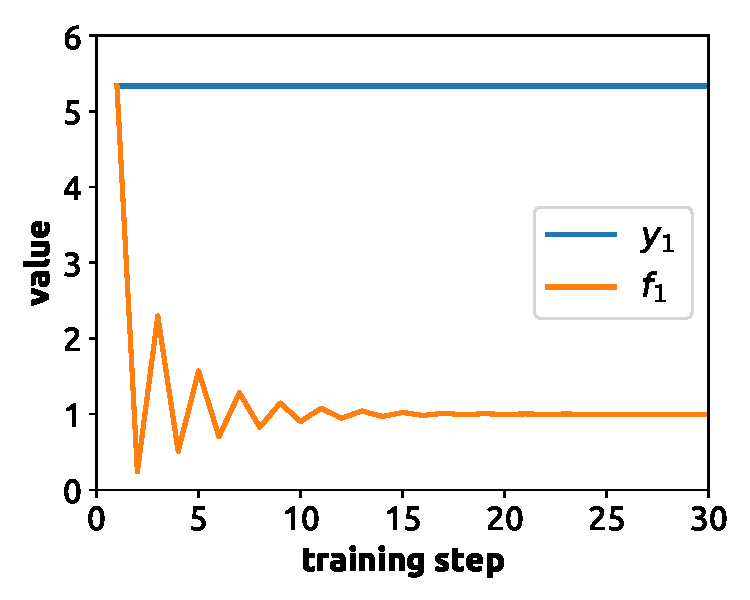
\includegraphics[width=0.9\columnwidth,trim={0 0.3cm 0 0},clip]{images/fig1.pdf}}
    \caption{The output value \texttt{y!} as a function of self-consistent training step.}\label{fig:invtrain}
\end{figure}

By viewing $\vx$ and parameters in $\vp_x$ as variables, we can study the trainability from the information perspective.
\begin{theorem}
    Only if the the conditional entropy $S(\vy|\vp_y)$ is nonzero, algorithm \ref{algo:train} is trainable.
\end{theorem}
\begin{proof}
The above example reveals a fact that training impossible when output parameters completely determines input parameters (or $S(\vp_x | \vp_y) = 0$).
\begin{align}
    \begin{split}
        S(\vp_x | \vp_y) &= S(\vp_x \cup \vp_y) - S(\vp_y)\\
        &\leq S\left((\vp_x \cup \vx) \cup \vp_y \right) - S(\vp_y),\\
        &\leq S\left((\vp_y \cup \vy) \cup \vp_y\right) - S(\vp_y),\\
    &\leq S(\vy|\vp_y).
    \end{split}
\end{align}
The third line uses the bijectivity $S(\vx \cup \vp_x) = S(\vy \cup \vp_y)$.
This inequality shows that when the parameter space on the output side satisfies $S(\vy | \vp_y) = 0$, i.e., contains all information to determine the output field, and the input parameters are also entirely determined by this parameter space. Hence training can not work.
\end{proof}
In the above example, it corresponds to the case $S\left(e^{(x+y)-e^x} | x \cup x + y\right) = 0$ in \texttt{f1}.
The solution is to remove the information redundancy in output parameter space through uncomputing, as shown in \texttt{f2}.
Besides, the Fibonacci example is often used in a reversible language as a tutorial, NiLang implementation could be found in \App{app:fib}.

\section{Functions used in the main text}\label{app:functions}

We list the functions used in \Sec{sec:example} as bellow.

\begin{minipage}{.44\textwidth}
\begin{lstlisting}
"""
get the summation of an array.
"""
@i function isum(out!, x::AbstractArray)
    for i=1:length(x)
        out! += identity(x[i])
    end
end

"""
computing factorial.
"""
@i function ifactorial(out!, n)
    out! += identity(1)
    for i=1:n
        mulint(out!, i)
    end
end

"""
dot product.
"""
@i function dot(out!, v1::Vector{T}, v2) where T
    for i = 1:length(v1)
        out! += v1[i]'*v2[i]
    end
end

"""
squared norm.
"""
@i function norm2(out!, vec::Vector{T}) where T
    anc1 ← zero(T)
    for i = 1:length(vec)
        anc1 += identity(vec[i]')
        out! += anc1*vec[i]
        anc1 -= identity(vec[i]')
    end
end

"""
Variance and mean value from squared values `sqv`.
"""
@i function var_and_mean_sq(var!, mean!, sqv)
    sqmean ← zero(mean!)
    @inbounds for i=1:length(sqv)
        mean! += sqv[i] ^ 0.5
        var! += identity(sqv[i])
    end
    divint(mean!, length(sqv))
    divint(var!, length(sqv))
    sqmean += mean! ^ 2
    var! -= identity(sqmean)
    sqmean -= mean! ^ 2
    mulint(var!, length(sqv))
    divint(var!, length(sqv)-1)
end
\end{lstlisting}
\end{minipage}

%In \texttt{norm2}, we copied \texttt{vec[i]\textquotesingle} to \texttt{anc1} to avoid the same variable appear twice in the argument list of $\oplus(*)$, where the prime represents the adjoint dataview.

\section{CUDA compitibility}\label{app:cuda}
CUDA programming is playing a more and more significant role in high-performance computing. In Julia, one can write kernel functions in native Julia language with CUDAnative~\cite{Besard2018}.
NiLang is compatible with CUDAnative and KernelAbstractions~\cite{KernelAbstractions}, and one can write a reversible kernel like the following.

\begin{minipage}{.44\textwidth}
\begin{lstlisting}
using CuArrays, CUDAnative, GPUArrays
using NiLang, NiLang.AD

@i @inline function swap_kernel(state, mask1, mask2)
    @invcheckoff begin
        b ← (blockIdx().x-1) * 
            blockDim().x + threadIdx().x - 1
        if (b < length(state), ~)
            if (b&mask1==0 && b&mask2==mask2, ~)
                SWAP(state[b+1], state[b ⊻ 
                    (mask1|mask2) + 1])
            end
        end
        b → (blockIdx().x-1) * 
            blockDim().x + threadIdx().x - 1
    end
end
\end{lstlisting}
\end{minipage}

This kernel function simulates the SWAP gate in quantum computing.
Here, one must use the macro \texttt{@invcheckoff} to turn off the reversibility checks. It is necessary because the possible error thrown in a kernel function can not be handled on a CUDA kernel.
One can launch this kernel function to GPUs with a single macro \texttt{@cuda}, as shown in the following using case.

\begin{minipage}{.44\textwidth}
\begin{lstlisting}
julia> @i function instruct!(state::CuVector,
            gate::Val{:SWAP}, locs::Tuple{Int,Int})
           mask1 ← 1 << (tget(locs, 1)-1)
           mask2 ← 1 << (tget(locs, 2)-1)
           XY ← GPUArrays.thread_blocks_heuristic(
                length(state))
           @cuda threads=tget(XY,1) blocks=tget(XY,
                2) swap_kernel(state, mask1, mask2)
       end

julia> instruct!(CuArray(randn(8)),
            Val(:SWAP), (1,3))[1]
8-element CuArray{Float64,1,Nothing}:
 -0.06956048379200473
 -0.6464176838567472
 -0.06523362834285944
 -0.7314356941903547
  1.512329204247244
  0.9773772766637732
  1.6473223915215722
 -1.0631789613639087
\end{lstlisting}
\end{minipage}

One can also write kernels with KernelAbstaction. It solves many compatibility issues related to different function calls on GPU and CPU.


\begin{minipage}{.44\textwidth}
\begin{lstlisting}
@i @kernel function swap_kernel2(state, mask1, mask2)
    @invcheckoff begin
        b ← @index(Global)
        if (b < length(state), ~)
            if (b&mask1==0 && b&mask2==mask2, ~)
                SWAP(state[b+1], state[b ⊻ 
                    (mask1|mask2) + 1])
            end
        end
        b → @index(Global)
    end
end
\end{lstlisting}
\end{minipage}

We can use the macro \texttt{@launchkernel} to launch a kernel.
The first parameter is a device.
The second parameter is the block size,
The third parameter is the number of threads.
The last parameter is a kernel function call to be launched.

\begin{minipage}{.44\textwidth}
\begin{lstlisting}
julia> @i function instruct!(state::CuVector,
            gate::Val{:SWAP}, locs::Tuple{Int,Int})
           mask1 ← 1 << (tget(locs, 1)-1)
           mask2 ← 1 << (tget(locs, 2)-1)
           XY ← GPUArrays.thread_blocks_heuristic(
                length(state))
           @launchkernel CUDA() 256 length(out!
                ) swap_kernel2(state, mask1, mask2)
       end

julia> instruct!(CuArray(randn(8)),
            Val(:SWAP), (1,3))[1]
8-element CuArray{Float64,1,Nothing}:
  2.1492759883720525 
  2.326837084303501  
  1.4587667131427016 
 -1.3273806428138293 
 -0.03975355575683114
 -0.10763082744447787
 -1.7111718557581195 
 -0.47922613687722704
\end{lstlisting}
\end{minipage}


\section{Computing Fibonacci Numbers}\label{app:fib}
The following is an example that everyone likes, computing Fibonacci number recursively.

\begin{minipage}{.44\textwidth}
    \begin{lstlisting}
using NiLang

@i function rfib(out!, n::T) where T
    n1 ← zero(T)
    n2 ← zero(T)
    @routine begin
        n1 += identity(n)
        n1 -= identity(1)
        n2 += identity(n)
        n2 -= identity(2)
    end
    if (value(n) <= 2, ~)
        out! += identity(1)
    else
        rfib(out!, n1)
        rfib(out!, n2)
    end
    ~@routine
end
\end{lstlisting}
\end{minipage}

The time complexity of this recursive algorithm is exponential to input \texttt{n}. It is also possible to write a reversible linear time with for loops.
A slightly non-trivial task is computing the first Fibonacci number that greater or equal to a certain number $z$, where a \texttt{while} statement is required.

\begin{minipage}{.44\textwidth}
\begin{lstlisting}
@i function rfibn(n!, z)
    @safe @assert n! == 0
    out ← 0
    rfib(out, n!)
    while (out < z, n! != 0)
        ~rfib(out, n!)
        n! += identity(1)
        rfib(out, n!)
    end
    ~rfib(out, n!)
end
\end{lstlisting}
\end{minipage}

In this example, the postcondition \texttt{n!=0} in the \texttt{while} statement is false before entering the loop, and becomes true in later iterations. In the reverse program, the \texttt{while} statement stops at \texttt{n==0}.
If executed correctly, a user will see the following result.

\begin{minipage}{.44\textwidth}
\begin{lstlisting}
julia> rfib(0, 10)
(55, 10)

julia> rfibn(0, 100)
(12, 100)

julia> (~rfibn)(rfibn(0, 100)...)
(0, 100)
\end{lstlisting}
\end{minipage}

This example shows how an addition postcondition provided by the user can help to reverse a control flow without caching controls.

\section{Alternative approaches to Obtain Hessian}\label{app:hessian}
This function itself is reversible and differentiable. Hence one can back-propagate this function to obtain Hessians as introduced in \Sec{sec:simplehessian}. In NiLang, it is implemented as \texttt{hessian\_backback}.

\begin{minipage}{.44\textwidth}
\begin{lstlisting}
julia> hessian_backback(ibesselj, (0.0, 2, 1.0);
            iloss=1)
3×3 Array{Float64,2}:
 0.0  0.0  0.0     
 0.0  0.0  0.0     
 0.0  0.0  0.134467
\end{lstlisting}
\end{minipage}

\begin{figure}[h]
    \centerline{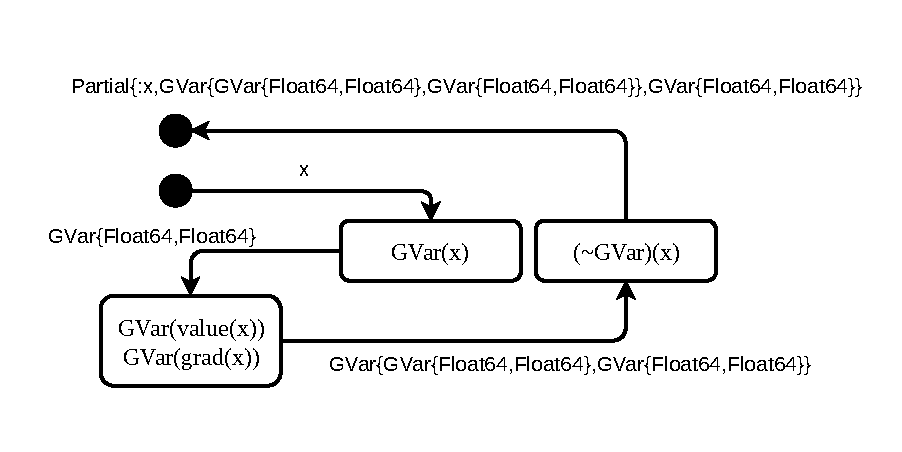
\includegraphics[width=\columnwidth,trim={0 1cm 0cm 1cm},clip]{images/simplehessian.pdf}}
    \caption{Data flow in obtaining second-order gradients with the recursive differentiation approach. Annotations on lines are data types used in the computation.}\label{fig:simplehessian}
\end{figure}

\Fig{fig:simplehessian} shows the data flow in the four passes of computing Hessian. The first two passes obtains the gradients. Before entering the third pass, the program wraps each field in \texttt{GVar} with another layer of \texttt{GVar}. Then we pick a variable $x_i$ and add $1$ to the gradient field of its gradient \texttt{grad(grad($x_i$))} in order to compute the $i$-th row of Hessian. Before entering the final pass, the \texttt{$\sim$GVar} is called. We can not unwrap \texttt{GVar} directly because although the values of gradients have been uncomputed to zero, the gradient fields of gradients may be nonzero. Instead, we use \texttt{Partial\{:x\}(obj)} to take field \texttt{x} of an object without erasing memory. By repeating the above procedure for different $x_i$, one can obtains the full Hessian matrix.

To obtain Hessians, we can also use the Hessian propagation approach as introduced in \Sec{sec:taylor}.

\begin{minipage}{.44\textwidth}
\begin{lstlisting}
julia> hessian_propagate(ibesselj, (0.0, 2, 1.0); iloss=1)
(BeijingRing{Float64}(0.0, 1.0, 1), 2,
    BeijingRing{Float64}(1.0, 0.21024361585934268, 2))

julia> collect_hessian()
2×2 Array{Float64,2}:
 0.0  0.0     
 0.0  0.134467
\end{lstlisting}
\end{minipage}

\texttt{ibesselj\textquotesingle\textquotesingle} computes the second-order gradients. It wraps variables with type \texttt{BeijingRing}~\footnote{When people ask for the location in Beijing, they will start by asking which ring it is? We use the similar approach to locate the elements of Hessian matrix.} in the backward pass. \texttt{BeijingRing} records Jacobians and Hessians for a variable, where Hessians are stored in a global storage.
Whenever an $n$-th variable or ancilla is created, we push a ring of size $2n-1$ to a global tape. Whenever an ancilla is deallocated, we pop a ring from the top. The $n$-th ring stores Hessian elements $H_{i\leq n,n}$ and $H_{n,i<n}$.% We didn't use the symmetry relation $H_{i,j} = H_{j,i}$ to save memory here in order to simplify the implementation of backward rules described in the right most panel of \Fig{fig:ad}.
The final result can be collected by calling \texttt{collect\_hessian()}, which will read out the Hessian matrix stored in the global storage.
This method turns out to allocate too much for ancillas, hence is not economic in practice.

\end{document}
